\documentclass[a4paper,11pt]{book}

\usepackage{graphicx}
\usepackage[T1]{fontenc}
\usepackage[utf8]{inputenc}
\usepackage{amsmath}
\usepackage{lmodern}
\usepackage{geometry}
\usepackage{amssymb}

\title{Solutions Guide to Y.A. Rozanov's Probability Theory: A Concise Course}
\author{Joseph Goodknight}
\date{Spring 2012}

\begin{document}

\maketitle


\chapter*{Introduction}

I found this delightful-looking probability theory textbook at a book sale at Harvard University's Cabot science library in the Spring of 2012.  I really wanted to learn the contents of the book and I figured the best way to do that would be to read it and solve the problems as I went along.

Throughout the course of the book, I indicate whether or not my answers have been verified by an outside source.  When the logic to the answer seems to be central to the solution even though I know that the answer I eventually get to is correct, I will indicate it as not being verified.  

Verification sources include the textbook and university course webpages.  Due credit will be made wherever possible.


\chapter{Basic Concepts}
\section{Important/Useful Theorems}
\subsection{Stirling's Formula}
\begin{equation}
	n! \approx \sqrt{2 \pi n} n^n e^{-n}
\end{equation}
\section{Answers to Problems}

%%answer template
%\subsection{}
%%problem n.n
%
%
%\begin{equation}
%	
%\label{answern.n}
%\end{equation}
%\textbf{Answer [not] verified}

\subsection{}
%problem 1.1
If you have four volumes, and the question is what order to place them in, the question is a simple permutation problem.  There are 4 possibilities for the first, 3 for the second, 2 for the third and only one for the last, making the number of permutations of the books 24.  Only one order has them in ascending order and only one order will have them in descending order.  Thus:
\begin{equation}
	P=\frac{2}{24}=\frac{1}{12}
\label{answer1.1}
\end{equation}
\textbf{Answer not verified}

\subsection{}
%problem 1.2
The wooden cube is made of $10^3$ cubes implying a 10x10x10 cube.  The cubes that have two faces painted will be the edges which are not on a corner.  Thus, since there are 12 edges of 10 cubes each, 8 of which are not corners, that implies we have 96 edges.  96 thus becomes our number of desireable outcomes and 1000 has always been the total number of outcomes:
\begin{equation}
	P=\frac{96}{1000} = 0.096
\label{answer1.2}
\end{equation}
\textbf{Answer verified}


\subsection{}
%problem 1.3

If there are $n$ total items and $k$ of them are defective.  We select $m$ and want to know the probability of $l$ of them being defective ones.

There are $\binom{n}{m}$ possible ways to chose $m$ different items from the population of $n$ items which will be our denominator.  Now we need to know how many of those possibilities have $l$ bad ones in them for our numerator.  If there's $k$ total defective ones, then there are $\binom{k}{l}$

\begin{equation}
	P = \frac{\binom{k}{l}}{\binom{n}{m}}
\label{answer1.3}
\end{equation}
\textbf{Answer not verified}


\subsection{}
%problem 1.4

There are $10!$ possible ways to order the ten books.  You can imagine that since the three books have to take up three adjacent positions, there are 8 possible locations for the three books to be ordered.  Taking just the first position (that being the first three ``Slots''), there are 6 ways to order the desired books and then $7!$ ways to order the remaining books.  Thus there are $8 \cdot{} 6 \cdot{} 7!$ desirable orders giving us a probability of

\begin{equation}
	P=\frac{8 \cdot{} 6 \cdot{} 7!}{10!}=\frac{1}{15}
\label{answer1.4}
\end{equation}
\textbf{Answer  verified}

%answer template
\subsection{}
%problem 1.5

There are 4 possibilities to consider here: neither hits, one or the other hits and both hits.  While it may be tempting to calculate the probability of each event, since we only care about the probability of at least one hitting the target, we need only calculate the probability that no one hits and subtract that from 1.  The first marksman has an $.8$ probability of hitting meaning he has a missing probability of .2; similarly the second marksman has a .7 chance of hitting and a .3 chance of missing.  Thus, the probability of both one and two missing is the product of the two missing probabilities: $.2*.3=.06$

\begin{equation}
	P=1-.06=.94
\label{answer1.5}
\end{equation}
\textbf{Answer verified}


\subsection{}
%problem 1.6
The total number of ways $n+k$ seats can be occupied by $n$ people is $\binom{n+k}{n}=\frac{(n+k)!}{n!k!}$ but once again the difficult part is finding the total number of desirable outcomes. If you were to specify $m$ seats, you effectively divide the auditorium into two buckets so we need to find the number of ways to partition people into those two buckets which will give us the numerator, $\binom{n+k}{m}=\frac{(n+k)!}{m!(n+k-m)!}$

\begin{equation}
	P=\frac{(n+k)!}{m!(n+k-m)!}\frac{n!k!}{(n+k)!}=\frac{{n!k!}}{m!(n+k-m)!}
\label{answer1.6}
\end{equation}
\textbf{Answer not verified}


\subsection{}
%problem 1.7

Again, the number of ways to get three cards from a 52 card deck is $\binom{52}{3}$.  Since there are 4 each of sevens, threes and aces, there are $4^3$ desirable hands.

\begin{equation}
	P=\frac{4^3}{\frac{52!}{3!49!}}=\frac{16}{5525}=0.00289593
\label{answer1.7}
\end{equation}
Which it is worth pointing out, is no different than any other 3-card hand of three different cards.
\textbf{Answer not verified}

\subsection{}
%problem 1.8
If you indiscriminately chose 3 line segments from our bank of 5, you have $\binom{5}{3}=10$ total possibilities for triangles.  When you look at the bank (1, 3, 5, 7, 9), however, you have to make sure that any two segments are longer than the third segment, otherwise making a triangle is impossible.  The brute-force way to do this is start with 1 and realize that no triangle can be formed with it.  Then, looking at 3, you realize that you can do (3, 5, 7) and (3, 7, 9).  Starting now with 5, you can do (5, 7, 9) but that's the only triangle that hasn't already been enumerated.  At this point, you realize you're done and that the answer is plain to see

\begin{equation}
	P=\frac{3}{10}=.3
\label{answer1.8}
\end{equation}
\textbf{Answer not verified}

\subsection{}
%problem 1.9

We could do this problem in 5 minutes of programming and an instant of computation but that's not the point!  We need to think our way through this one.  How many cubes of the numbers between 1 and 1000, have 11 for the last two digits.  Luckily, each cube is unique so there's no complications there: only 1000 possibilities.  

Let's break down the number we're cubing into two parts, one that encapsulates the part less than 100 and then the rest of the number
\begin{equation}
	n=a+b=100c+b
\end{equation}
Now, just for fun, let's cube than number
\begin{equation}
	n^3=(100c+b)^3=b^3+300 b^2 c+30000 b c^2+1000000 c^3
\end{equation}
Clearly the only term here that will matter to the last two digits of the cube is $b$, the part less than 100.  Now we can reduce our now size 100 subspace by a great deal if you realize that in order for a number's cube to end in 1, the last number in the cube will need to be 1, leaving us: (1, 11, 21, 31, 41, 51, 61, 71, 81, 91).  At this point I recommend just cubing all the numbers and realizing that only $71^3=357911$ fulfills the requirements giving only one desirable outcome per century(71, 171, 271 etc.)

\begin{equation}
	P=\frac{10}{1000}=.01
\label{answer1.9}
\end{equation}
\textbf{Answer verified}

\subsection{}
%problem 1.10
Now we want to know about all positive integers but just the last digit and the probability that the last digit is one.  To prove that we can use the hint given, we'll split the integer into the past less than 10 and the part greater than 10.
\begin{equation}
	n=10a+b
\end{equation}
\subsubsection{a--Squared}
\begin{equation}
	n^2=100a^2+10ab+b^2
\end{equation}
OK, so clearly only $b^2$ contributes to the last digit.  At this point... just do the squaring especially since it's something you can do in your head. (1, 2, 3, 4, 5, 6, 7, 8, 9)$\rightarrow$(1, 4, 9, 16, 25, 36, 49, 64, 81) therefore there are two desireable outcomes for every decade of random positive integers.
\begin{equation}
	P=\frac{2}{10}=.2
\label{answer1.10a}
\end{equation}

\subsubsection{b--fourth-powered}
\begin{equation}
	n^4=100000000 a^4+4000000 a^3 b+60000 a^2 b^2+400 a b^3+b^4
\end{equation}
Great, once again, just $b^4$.  Now, doing the forth power is a little harder so let's reason through and reduce the subspace.  Clearly, only odd numbers will contribute since any power of an even number is again an even number. Now, let's just do the arithmetic. (1, 3, 5, 7, 9)$\rightarrow$(1, 81, 625, 2401, 6561) giving us 4 desirable outcomes per decade of random numbers
\begin{equation}
	P=\frac{4}{10}=.4
\label{answer1.10a}
\end{equation}

\subsubsection{b--multiplied by random positive number}
\begin{equation}
	n*r=(10a+b)r
\end{equation}
Now let's let $r$ be a similar integer as n
\begin{equation}
	n*r=(10a+b)(10c+d)=100ac+10(bc+ad)+bd
\end{equation}

So we just need to consider the first two digits of both the random number and the arbitrary number.  This leaves us with $10^2$ possibilities; $5^2$ possible desirable outcomes once we exclude even numbers: (1, 3, 5, 7, 9).  Once again we resort to brute force by just defining the above as a vector and multiplying the transpose of that vector by the vector.  The only desirable outcomes turn out to be (1*1, 9*9, 7*3, 3*7), giving four desirable outcomes per century.

\begin{equation}
	P=\frac{4}{100}=.04
\label{answer1.10b}
\end{equation}

\textbf{Answers all verified}

\subsection{}
%problem 1.11
Here we are given 8 possible numbers (2, 4, 6, 7, 8, 11, 12, 13) and are told that it making a random fraction out of two of the numbers.  There are $\binom{8}{2}=28$ possible pairs but since $\frac{a}{b} \neq \frac{b}{a}$, we multiply that by two to get the total number of fractions we can get from these numbers as being 56.  

Looking at the numbers given, 7, 11 and 13 are all prime and all the others are divisible by two; therefore only the fractions that contain one or more prime numbers will be in lowest terms.  The number 7 can be in 7 different pairs with the other numbers which makes for 14 fractions.  11 can be in 6 pairs or 12 fractions (since we already counted 7) and similarly, 13 can be in 10 uncounted fractions giving 36 possible fractions in lowest terms.

\begin{equation}
	P=\frac{36}{56}=\frac{9}{14}
\label{answer1.11}
\end{equation}
\textbf{Answer verified}

\subsection{}
%problem 1.12
The word drawer has 6 letters and there are $6!=720$ possible ways of arranging the letters.  It is then natural to say there's only one way to spell reward correctly and thus the probability of spelling it correctly after a random reordering is $1/720$ BUT there is a complication in that the two of our letters are the same, meaning there are to distinct arrangement of our distinguishable tiles that will give us the proper spelling.

\begin{equation}
	P=\frac{2}{720} = \frac{1}{360}
\label{answer1.12}
\end{equation}
\textbf{Answer verified}

\subsection{}
%problem 1.13
For any die, there are 6 different possibilities.  Since one dice's outcome does not depend on another's, that means that for a roll of $6n$ die, there are $6^{6n}$ different possible outcomes for the dice rolls.  

Now for desirable outcomes, we want each of the 6 faces to show up n times.  To accomplish this, we just count the number of ways to apportion $6n$ things into 6 groups of $n$ each or
\begin{equation}
	\frac{(6n)!}{(n!)^6}
\end{equation}
which, given Stirling's approximation
\begin{equation}
	n! \approx \sqrt{2 \pi n} n^n e^{-n}
\end{equation}
gives us for large $n$
\begin{equation}
	\frac{(6n)!}{(n!)^6} \approx \sqrt{2 \pi 6n} (6n)^{6n} e^{-6n} * \frac{1}{(\sqrt{2 \pi n} n^n e^{-n})^6} = \frac{3 \cdot 6^{6n}}{4 (\pi n)^{5/2}}
\end{equation}

\begin{equation}
	P=\frac{(6n)!}{(n!)^6 6^{6n}} \approx \frac{3}{4 (\pi n)^{5/2}}
\label{answer1.13}
\end{equation}
\textbf{Answer verified}



\subsection{}
%problem 1.14
To figure out the total number of possibilities, we must realize that one draw of half a deck, implies the other half of the deck implicitly, therefore there are $\binom{52}{26}$ total 26 card draws.  Then, to get 13 red cards, there are $\binom{26}{13} = 10400600$ ways to get 13 red cards and the same number for black cards making $10400600^2$ the number of total possible desirable outcomes.

\begin{equation}
	P=\frac{16232365000}{74417546961}=0.218126
\label{answer1.14}
\end{equation}
Because we're cool and modern and have Mathematica, we don't NEED to do the Stirling's formula approximation but it'll be good for us so we shall.
\begin{equation}
	P=\frac{\binom{26}{13}^2}{\binom{52}{26}} = \frac{(26!)^4}{(13!)^4 52!}=\frac{((2n)!)^4}{(n!)^4 (4n)!}
\end{equation}
where $n=13$.
\begin{equation}
	P=\frac{(\sqrt{4 \pi n}(2n)^{2n}e^{-2n})^4}{(\sqrt{2 \pi n}n^{n}e^{-n})^4 (\sqrt{8 \pi n}(4n)^{4n}e^{-4n})}
\end{equation}
\begin{equation}
	P=\frac{(4 \pi n)^2}{(2 \pi n)^2 \sqrt{8 \pi n}} \frac{(2n)^{8n}}{n^{4n}(4n)^{4n}} = \frac{4}{\sqrt{8 \pi n}} \frac{2^{8n}}{4^{4n}}
\end{equation}
\begin{equation}
	P=\frac{2}{\sqrt{26 \pi}} = 0.221293
\end{equation}
which when you take the ratio of approximate to exact, you get $1.01452$ so the approximation is less than $2\%$ off... not bad!

\textbf{Answer verified}

\subsection{}
%problem 1.15
There are 100 senators at any given time.  Much like the previous problem, there are $\binom{100}{50}=100891344545564193334812497256$ different 50 senator committees.  Much like the previous problem, there are $\binom{2}{1}=2$ ways for California to be represented on the committee making for 50 states $2^{50}$ possible even committees

\begin{equation}
	P=\frac{2^{50}}{\binom{100}{50}} = \text{1.115952921347132$\grave{ }$*${}^{\wedge}$-14}
\label{answer1.15}
\end{equation}
\textbf{Answer verified}

\subsection{}
%problem 1.16
For $2n$ people, there are $(2n)!$ different possible lines; we want the number of lines where at any given point in the line, there are more people with 5 dollar bills than 10 dollar bills.

The given reference (freely available on Google books) has a fascinating geometrical argument about how $\binom{2n}{n+1}$ is the number of lines that have one or more too many people with tens in front of people with fives.  Also, in this argument, there are $\binom{2n}{n}$ trajectories instead of $(2n)!$ lines.

\begin{equation}
	P=\frac{\binom{2n}{n}-\binom{2n}{n+1}}{\binom{2n}{n}} = \frac{1}{n+1}
\label{answer1.16}
\end{equation}
\textbf{Answer verified}

\subsection{}
%problem 1.17
We wish to prove that

\begin{equation}
	\sum_{k=0}^{n} \binom{n}{k}^2 = \binom{2n}{n}
\label{answer1.17}
\end{equation}

This is easies if we listen to the hint and consider that $\binom{2n}{n}$ is the coefficient of $x^n$ in the polynomial $(x+1)^{2n}$ which is also equivalent to $(x+1)^n(x+1)^n$

We make use of:
\begin{equation}
	(x+1)^n = \sum_{k=0}^{n} \binom{n}{k} x^k
\end{equation}
\begin{equation}
	(x+1)^n(x+1)^n = \sum_{k=0}^{n}\sum_{j=0}^{n} \binom{n}{k} \binom{n}{j} x^k x^j
\end{equation}
We want the $x^n$ term: where $k+j=n$ or, put another way, where $k=n-j$...
\begin{equation}
	\sum_{j=0}^{n} \binom{n}{n-j} \binom{n}{j} = \sum_{j=0}^{n} \frac{n!}{j!(n-j)!}\frac{n!}{(n-j)!j!} = \sum_{j=0}^{n} \binom{n}{j}^2
\end{equation}
QED


\textbf{Answer not verified}


%%answer template
%\subsection{}
%%problem n.n
%
%
%\begin{equation}
%	
%\label{answern.n}
%\end{equation}
%\textbf{Answer [not] verified}



\chapter{Combination of Events}

\section{Important/Useful Theorems}

\subsection{}
If $A_1 \subset A_2$ then $\bar{A_1} \supset \bar{A_2}$

\subsection{}
If $A = A_1 \cup A_2$ then $\bar{A} = \bar{A_1} \cap \bar{A_2}$

\subsection{}
If $A = A_1 \cap A_2$ then $\bar{A} = \bar{A_1} \cup \bar{A_2}$

\subsection{}
$0\leq P(A) \leq 1$

\subsection{}
$P(A_1 \cup A_2) = P(A_1) + P(A_2) - P(A_1 \cap A_2 )$

\subsection{}

$P(A_1) \leq P(A_2)$ if $A_1 \subset A_2$

\subsection{}
Given any $n$ events $A_1, A_2, ... A_n$, let
\begin{equation}
	P_1 = \sum_{i=1}^{n} P(A_i)
\end{equation}
\begin{equation}
	P_2 = \sum_{1 \leq i < j \leq n} P(A_iA_j)
\end{equation}
\begin{equation}
	P_3 = \sum_{1 \leq i < j < k \leq n} P(A_i A_j A_k)
\end{equation}
etc. for integers up to $n$.  Then
\begin{equation}
	P\left(\bigcup_{k=1}^n A_k \right) = P_1 -P_2 + P_3 + ... \pm P_n
\end{equation}

\subsection{}
If $A_1, A_2, ...$ is an increasing sequence of events such that $A_1 \subset A_2 \subset ...$
\begin{equation}
	P\left(\bigcup_{k=1}^n A_k \right) = \lim_{n \rightarrow \infty} P(A_n)
\end{equation}

\subsection{}
If $A_1, A_2, ...$ is an decreasing sequence of events such that $A_1 \supset A_2 \supset ...$
\begin{equation}
	P\left(\bigcap_{k=1}^n A_k \right) = \lim_{n \rightarrow \infty} P(A_n)
\end{equation}


\subsection{}
For any collection of arbitrary events
\begin{equation}
	P\left(\bigcup_{k} A_k \right) \leq \sum_k P(A_k)
\end{equation}

\subsection{}
For any sequence of events $A_1, A_2, ...$ with porbabilities $P(A_k)=p_k$
\begin{equation}
	\sum_k p_k < \infty
\end{equation}

\section{Answers to Problems}

%%answer template
%\subsection{}
%%problem n.n
%
%
%\begin{equation}
%	
%\label{answern.n}
%\end{equation}
%\textbf{Answer [not] verified}


\subsection{}
%problem 2.1
\subsubsection{a--$AB=A$}
$AB=A$ is shorthand for $A\cap B=A$ or, in English, that the intersection of the events $A$ and $B$ is equivalent to the event $A$.  Clearly, this means that $A$ is equivalent to $B$ such that their overlap is complete--wither because they are exactly the same or because all outcomes in B are contained in A
\subsubsection{b--$ABC=A$}

The intersection $A$, $B$ and $C$ is equivalent to A. This implies that both $B$ and $C$ are either the same as $A$ or contained within $A$

\subsubsection{c--$A\cup B\cup C=A$}

The intersection of $A$, $B$ and $C$ is equivalent to $A$.  This statement implies that the overlap of $B$ and $C$ is $A$.  

\textbf{Answer not verified}


\subsection{}
%problem 2.2
\subsubsection{a--$A \cup B = \bar{A}$}

The union of $A$ and $B$ is the complement of $A$.  This statement seems to imply that the sum of the events in both $A$ and $B$ are the same as the events NOT in A.  This seeming contradiction can only be true if $A$ as a set contains no events and $B$ contains all events.


\subsubsection{b--$AB=\bar{A}$}

The intersection of $A$ and $B$ is equivalent to the complement of $A$.  This statement implies that the events contained in both $A$ and $B$ are the events NOT in $A$.  Again, this strange statement can be fulfilled if $A$ contains all events and $B$ contains no events 

\subsubsection{c--$A \cup B = A \cap B$}

The union of $A$ and $B$ is equal to the intersection of $A$ and $B$.  This statement implies that the sum of all events in $A$ and $B$ is equivalent to the events in both $A$ and $B$.  This can be true, if $A=B$.

\textbf{Answer not verified}


\subsection{}
%problem 2.3
\subsubsection{a--$(A \cup B)(B \cup C)$}

In order to do this problem, we need to develop a distributive law for $\cap$ and $\cup$; we need to figure out what $A \cup (B \cap C)$ and $A \cap (B \cup C)$ is.

$A \cup (B \cap C)$ is the union of A and the intersection of $B$ and $C$ which one can easily imagine is the same as the union of the intersection of the union of $A$ and $B$, and $A$ and $C$.  

\begin{equation}
	A \cup (B \cap C) = (A \cup B) \cap (A \cup C)
\end{equation}
similarly, for the second relation
\begin{equation}
	A \cap (B \cup C) = (A \cap B) \cup (A \cap C)
\end{equation}

ALRIGHT  Back to the problem at hand
\begin{equation}
	(A \cup B) \cap (B \cup C)=D
\end{equation}
For bookkeeping purposes, I have defined our expression to equal $D$.  Let's distribute...
\begin{equation}
	(A \cap B) \cup (A \cap C)\cup (B \cap B)\cup (B \cap C)
\end{equation}
clearly the intersection of $B$ and $B$ is just $B$
\begin{equation}
	(A \cap B) \cup (A \cap C)\cup B \cup (B \cap C)
\end{equation}
let's rearrange it to look like what we want to prove (cheap move, I know... but effective!).
\begin{equation}
	(AC\cup B) \cup \left[(A \cap B) \cup (B \cap C)\right]=D
\end{equation}
If we could prove that the term in brackets is equal to $D$ then we would prove that $AC\cup B=D$.  So let's work on that:
\begin{equation}
	(A \cap B) \cup (B \cap C) = E
\end{equation}
Now let's distribute
\begin{equation}
	(A \cup B) \cap (B \cup C) \cap (B \cup B)\cap (A \cup C) = E
\end{equation}
simplify and rearrange
\begin{equation}
	\left[(A \cup B) \cap (B \cup C)\right] \cap B\cap (A \cup C) = E
\end{equation}
we recognize that the term in brackets is equivalent to the original expression we're trying to work with and then distribute one last time
\begin{equation}
	D \cap \left[(B \cap A) (B \cap C)\right] = E
\end{equation}
Now the term in brackets is equal to event $E$ meaning that $D=E$!  So we go back to the first equation.
\begin{equation}
	(AC\cup B) \cup D = D
\end{equation}
\begin{equation}
	(AC\cup B) = D = (A \cup B) \cap (B \cup C)
\end{equation}
$\Box$

\textbf{Answer not verified}

\subsubsection{b--$(A \cup B)(A \cup \bar{B})$}
\begin{equation}
	(A \cup B)\cap (A \cup \bar{B})
\end{equation}
distribute out
\begin{equation}
	(A \cap A)\cup (A \cap \bar{B})\cup (B \cap A)\cup (B \cap \bar{B})
\end{equation}
$A$ will intersect with itself only at itself and $B$ will not intersect with its copmlement.
\begin{equation}
	A\cup (A \cap \bar{B})\cup (B \cap A)\cup 0
\end{equation}
Unionizing the null set with anything else will leave the other things untouched.
\begin{equation}
	A\cup (A \cap \bar{B})\cup (B \cap A)
\end{equation}
Now we rearrange and redistribute.
\begin{equation}
	A\cup \left[  (A \cup A) \cap (A \cup B) \cap (A \cup \bar{B}) \cap (B \cup \bar{B}) \right]
\end{equation}
Clearly the sum of things in $B$ and not in $B$ is everything.
\begin{equation}
	A\cup \left[  A \cap (A \cup B) \cap (A \cup \bar{B}) \cap \Omega \right]
\end{equation}
Clearly the intersection of anything with everything is the same anything
\begin{equation}
	A\cup \left[  A \cap (A \cup B) \cap (A \cup \bar{B}) \right]
\end{equation}
Distribute.
\begin{equation}
	(A\cup A) \cap \left[  A \cup (A \cup B) \right]\cap \left[  A \cup (A \cup \bar{B}) \right]
\end{equation}
\begin{equation}
	A \cap \left[  (A \cup A) \cup B \right]\cap \left[  (A \cup A) \cup \bar{B} \right]
\end{equation}
\begin{equation}
	A \cap \left[  A \cup B \right]\cap \left[ A \cup \bar{B} \right]
\end{equation}
Now we call the original statement of the problem event $C$
\begin{equation}
	A \cap C = C
\end{equation}
Which as we discussed in problem 2.1a, implies that $A=C$.  Therefore:
\begin{equation}
	(A \cup B)(A \cup \bar{B}) = A
\label{answer2.3b}
\end{equation}
$\Box$

\textbf{Answer not verified}

\subsubsection{c--$(A \cup B)(A \cup \bar{B})(\bar{A} \cup B)$}
Start from the identity we just proved
\begin{equation}
	(A \cup B)(A \cup \bar{B})(\bar{A} \cup B) = A \cap (\bar{A} \cup B)
\end{equation}
Distribute
\begin{equation}
	(A \cap \bar{A}) \cup (A \cap B)
\end{equation}
\begin{equation}
	0 \cup AB
\end{equation}
\begin{equation}
	AB
\end{equation}
$\Box$

\textbf{Answer not verified} 

\subsection{}
%problem 2.4
Solve for $X$:
\begin{equation}
	\overline{(X \cup A)} \cup \overline{(X \cup \overline{A})} = B
\end{equation}
We negate both sides and use DeMorgan's theorem
\begin{equation}
	(X \cup A) \cap (X \cup \overline{A}) = \overline{B}
\end{equation}
Since we just fought so hard to prove that $(A \cup B)(B \cup C) = AC \cup B$, we want to use it!
\begin{equation}
	(A \cup X) \cap (X \cup \overline{A}) = \overline{B}
\end{equation}
\begin{equation}
	(A \overline{A}) \cup X = \overline{B}
\end{equation}
\begin{equation}
	0 \cup X = \overline{B}
\end{equation}
\begin{equation}
	X = \overline{B}
\end{equation}
$\Box$

\textbf{Answer not verified}


\subsection{}
%problem 2.5

$A$ is the event that at least one of three inspected items is defective and $B$ is the event that all three inspected items are defective.  In this circumstance, the overlap of $A$ and $B$ ($A \cap B$) is equal to $A$ since $A \subset B$.  For similar reasons, the union of those two ($A \cup B$) is simply equal to $B$.


\textbf{Answer not verified}

\subsection{}
%problem 2.6

Since $B$ is the event a number ends in a zero, $\overline{B}$ is the event a number does not end in a zero.  Thus, the overlap of that event and a number being divisible by 5 is the same as saying the event that a number is divisible by 5 and not divisible by 10.


\textbf{Answer not verified}

\subsection{}
%problem 2.7

It is easy to prove to oneself that these events $A_k$ are increasing such that $A_1 \subset A_2 \subset A_3 \subset A_4 \subset ... \subset A_10$ since the radii of the disks are getting bigger.  Therefore, according to theorem 2.3 from the text
\begin{equation}
	B = \bigcup_{k=1}^6 A_k = A_6
\end{equation}
Intuitively, this is clear because we're taking the $A_6$ contains all the lower events so if you take the union of all the lower events then you're just adding parts of $A_6$ to itself.  Now, for
\begin{equation}
	C = \bigcap_{k=5}^{10} A_k
\end{equation}
will clearly be $A_5$ because it's the smallest event and thus automatically sets the intersection to not be able to be any smaller.

\textbf{Answer verified}


\subsection{}
%problem 2.8
Luckily with just a bit of work, we can prove that the two statements are equivalent
\begin{equation}
	P(A) + P(\overline{A}) = 1
\end{equation}
To prove this, we'll use the probability addition theorem for two events which will be $A$ and $\overline{A}$ for us.
\begin{equation}
	P(A \cup B) = P(A) + P(B) - P(A \cap B)
\end{equation}
substitute:
\begin{equation}
	P(A \cup \overline{A}) = P(A) + P(\overline{A}) - P(A \cap \overline{A})
\end{equation}
using the fact that the union of anything with everything else is everything and that the intersection of anything with anything else is nothing...
\begin{equation}
	P(\Omega) = P(A) + P(\overline{A}) - P(0)
\end{equation}
Now we use the fact that the probability of ell events is unity and the probability of no events is nothing.
\begin{equation}
	1 = P(A) + P(\overline{A}) - 0
\end{equation}
$\Box$

\textbf{Answer not verified}


\subsection{}
%problem 2.9

I think this problem is as easy as it sounds since they're very clear to label the probabilities as belonging to the rings and the disk.  Thus, if you draw a picture of the bulls-eye it will become clear that the answer is just $1-.35-.30-.25=.10$ probability of missing.
\textbf{Answer not verified}

\subsection{}
%problem 2.10

Let $A_i$ be the event where $i$ or fewer defective items are found; we're looking, then for the event $B$ that we find at least one defective item:
\begin{equation}
	B = \bigcup_{i=1}^5 A_i
\end{equation}
\begin{equation}
	P(B) = P \left( \bigcup_{i=1}^5 A_i  \right)
\end{equation}
Consequently
\begin{equation}
	P(\overline{B}) = P \left( \bigcup_{i=1}^5 \overline{A_i}  \right)
\end{equation}
Clearly $A_i$ are an increasing series of events so consequently, $\overline{A_i}$ are a decreasing series of events and we can use theorem 
\begin{equation}
	P(B) = 1- P(\overline{B}) = 1- P ( \overline{A_5} )
\end{equation}

This is saying the probability of rejecting the batch that has 5 bad items in it is 1 minus the probability of not finding 5 or fewer bad items: or of finding 5 good items.

There are $\binom{100}{5}$ ways to pick 5 items from 100.  With 95 good items, there are $\binom{95}{5}$ ways to pick up 5 good items.
\begin{equation}
	P = 1 - \frac{\binom{95}{5}}{\binom{100}{5}} = 1 - \frac{95!}{5! \cdot 90! } \frac{95! \cdot 5!}{100!} = 1 - \frac{95!}{90! } \frac{95!}{100!}
\end{equation}
\begin{equation}
	P = 1 - \frac{95\cdot 94\cdot 93\cdot 92\cdot 91}{100 \cdot 99\cdot 98\cdot 97\cdot 96} = \frac{2478143}{10755360} = 0.23041
\label{answer2.10}
\end{equation}
\textbf{Answer verified}

\subsection{}
%problem 2.11

This problem boils down to the game you may have played as a kid to decide who got to go first or ride in the front of the car: I'm thinking of a number between 1 and 10.  Granted here the secretary gets to guess until she gets it right.  Let $A_i$ be the event that the secretary guesses just $i$ times (gets it right on the $i$th try). Thus we want:
\begin{equation}
	P(B) = P\left(\bigcup_{i=1}^4 A_i \right) = \sum_{i=1}^4 P(A_i)
\end{equation}
This factorization brought to you by the letter 'I` and the fact that you can't simultaneously get it right on the first try and get it right on the second try, meaning these events are mutually exclusive.  

For $i$ trials, there are $P^{10}_i$ possible ways to have tried.  Note that here order matters since we're talking about successive trials.  Consequently, there are $P^9_{i-1}$ ways to chose $i-1$ wrong numbers, giving
\begin{equation}
	P_i=\frac{P^9_{i-1}}{P^{10}_i}=\frac{1}{10}
\end{equation}
This answer, in itself, makes some sense although it does, at first glance, appear weird since you expect to gain an advantage as you learn about which numbers aren't correct.  In reality, there's 10 possible chances to get it right and you're no more likely to get it right on the first than on the second etc.; that's the best intuitive way to think about it.
\begin{equation}
	P(B) = \sum_{i=1}^4 \frac{1}{10} = .4
\end{equation}
Now, if the secretary knew that the last number had to be even, that reduces our total number of possible numbers to 5 so the probability becomes:
\begin{equation}
	P_i=\frac{P^4_{i-1}}{P^{5}_i}=\frac{1}{5}
\end{equation}
so instead we get
\begin{equation}
	P(B) = \sum_{i=1}^4 \frac{1}{5} = .8
\end{equation}

\textbf{Answer not verified}


\subsection{}
%problem 2.12
We proved earlier that $P(A) = 1 - P(\overline{A})$ so if we define

\begin{equation}
	B = \bigcup_{k=1}^n A_k
\end{equation}
then we know
\begin{equation}
	\overline{B} = \bigcap_{k=1}^n \overline{A_k}
\end{equation}
and thus
\begin{equation}
	1 - P\left(\bigcup_{k=1}^n A_k\right)  =P\left( \bigcap_{k=1}^n \overline{A_k} \right)
\end{equation}
$\Box$

\textbf{Answer not verified}

\subsection{}
%problem 2.13

Here we need to find the probability that you get 5 good ones and the probability you get one bad one; their sum will be the probability that the batch passes.

For both probabilities, the total number of outcomes is equal to the total number of groups of 50 objects out of the 100 or $\binom{100}{50} = 100891344545564193334812497256$.

For finding 5 good ones, there $\binom{95}{50}$ ways to pick 50 good ones.  Additionally, there's $\binom{95}{49}\binom{5}{1}$ to get 49 good ones and one bad one.

\begin{equation}
	P = \frac{\binom{95}{50}+\binom{95}{49}\binom{5}{1}}{\binom{100}{50}} = \frac{1739}{9603} = 0.181089
\label{answer2.13}
\end{equation}
\textbf{Answer verified}

\subsection{}
%problem 2.14

To solve this problem, you want to consider the people as buckets and the birthdays as things you put in the buckets.  As such, there are $365^r$ different possible ways for people to r people to have birthdays.  

In order to get the probability that at least one person shares a birthday, like we proved for the earlier problem, we need to just find the probability that no one shares a birthday and subtract that from 1.  

For the first person, there are 365 possibilities, 364 for the next, ad nauseum, giving $P^{365}_r$ ways of no one sharing a birthday.

\begin{equation}
	P(r) = 1 - \frac{P^{365}_r}{365^r} = 1 - \frac{365!}{365^r(365-r)!}
\label{answern2.14}
\end{equation}
\textbf{Answer verified by wikipedia}

\subsection{}
%problem 2.15

We are asked to check how good the truncation of
\begin{equation}
	1-e^x = -\sum_{n=1}^\infty \frac{x^n}{n!}
\end{equation}
is for $n=3, 4, 5, 6$ at $x=-1$.  
\begin{equation}
	1-e^{-1} = 0.632121 \approx 1 - \frac{1}{2} + \frac{1}{6} - \frac{1}{24}  + \frac{1}{120} - \frac{1}{720} 
\end{equation}
These truncations go as: $\{0.666667,0.625,0.633333,0.631944\}$ which relative to the exact answer are $\{1.05465,0.988735,1.00192,0.999721\}$


\textbf{Answer not verified}

\subsection{}
%problem 2.16

Here we have 4 events to look at: the probability that each player gets dealt a hand of one suit.  
\begin{equation}
	P_1 = P(A_1) + P(A_2) + P(A_3) + P(A_4) = 4P(A_i)
\end{equation}
\begin{equation}
	P_2 = P(A_1 A_2) + P(A_1 A_3) + P(A_1 A_4) + P(A_2 A_3) + P(A_2 A_4) + P(A_3 A_4) = 6 P(A_i A_j)
\end{equation}
because each one of these is equivalent to the others (player 2 and 3 getting full hands is no more likely than player 4 and 1).  
\begin{equation}
	P_3 = P(A_1 A_2 A_3) + P(A_1 A_2 A_4) + P(A_1 A_3 A_4) + P(A_2 A_3 A_4) = 4 P(A_i A_j A_k)
\end{equation}
\begin{equation}
	P_4 = P(A_1 A_2 A_3 A_4)
\end{equation}

For one player's hand, there are $\binom{52}{13}$ possibilities, only 4 of which are all the same suit.  For two players, the first player once again has $\binom{52}{13}$ possibilities but that leaves only $\binom{39}{13}$ for the second player (and $\binom{26}{13}$ for the third) giving a total number of hands for two players as $\binom{52}{13}\binom{39}{13}$ and $\binom{52}{13}\binom{39}{13}\binom{26}{13}$ for 3/4 players.

For 2 players, there are 4 possible hands for the first, leaving 3 for the second and giving 12 total desirable hands.  Consequently for three players, there are two more options giving 24 total desirable hands.


\begin{equation}
	P_1 =  4\left(\frac{4}{\binom{52}{13}}\right)
\end{equation}
\begin{equation}
	P_2 = 6\left( \frac{12}{\binom{52}{13}\binom{39}{13}} \right)
\end{equation} 
\begin{equation}
	P_3 = 4\left( \frac{24}{\binom{52}{13}\binom{39}{13}\binom{26}{13}} \right)
\end{equation}
\begin{equation}
	P_4 = \frac{24}{\binom{52}{13}\binom{39}{13}\binom{26}{13}}
\end{equation}
\begin{equation}
	P\left(A_1 \cup A_2 \cup A_3 \cup A_4\right) = P_1 - P_2 +P_3 - P_4
\end{equation}
\begin{equation}
	P\left(A_1 \cup A_2 \cup A_3 \cup A_4\right) = \frac{16}{\binom{52}{13}} - \frac{72}{\binom{52}{13}\binom{39}{13}} + \frac{72}{\binom{52}{13}\binom{39}{13}\binom{26}{13}}
\label{answer2.16}
\end{equation}
because I have mathematica and I'm feeling lazy at the moment, I am just going to forgo the Stirling's Approximation part and tell you:
\begin{equation}
	P\left(A_1 \cup A_2 \cup A_3 \cup A_4\right) = \frac{18772910672458601}{745065802298455456100520000} \approx 2.5196312345 \cdot 10^{-11}
\end{equation}


\textbf{Answer verified}

\subsection{}
%problem 2.17

SKIPPED

\begin{equation}
	0=0
\label{answer2.17}
\end{equation}
\textbf{Answer [not] verified}

\subsection{}
%problem 2.18

SKIPPED

\begin{equation}
	0=0
\label{answer2.18}
\end{equation}
\textbf{Answer [not] verified}

\subsection{}
%problem 2.19

SKIPPED

\begin{equation}
	0=0
\label{answer2.19}
\end{equation}
\textbf{Answer [not] verified}






%%answer template
%\subsection{}
%%problem n.n
%
%
%\begin{equation}
%	
%\label{answern.n}
%\end{equation}
%\textbf{Answer [not] verified}








\chapter{Combination of Events}

\section{Important/Useful Theorems}

\subsection{}

\begin{equation}
	P(A|B) = \frac{P(AB)}{P(B)}
\end{equation}

\subsection{}
If $A = \bigcup{}_k A_k$ where $A_k$ are all mutually exclusive
\begin{equation}
	P(A|B) = \sum_k P(A_k|B)
\end{equation}

\subsection{}
The events $A_1, A_2, A_3, ..., A_n$ are said to be statistically independent if
\begin{eqnarray*}
	P(A_i A_j) = P(A_i)P(A_j) \\
	P(A_i A_j A_k) = P(A_i)P(A_j)P(A_k) \\
	... \\
	P(A_1 A_2 A_3...A_n) = P(A_1)P(A_2)P(A_3)...P(A_n)
\end{eqnarray*}
For all possible combinations of the indeces.

\subsection{Second Borel-Cantelli lemma}
If the events $A_1, A_2, A_3, ...$ are all statistically independent and $p_k = P(A_k$
\begin{equation}
	\sum_{k=1}^\infty p_k = \infty
\end{equation}


\section{Answers to Problems}

%answer template
\subsection{}
%problem 3.1

We need to examine $A(\bar{A}B)$ , $A \overline{A \cup B}$ and $(\bar{A}B) \overline{A \cup B}$.

\begin{equation}
	A(\bar{A}B) = A\bar{A}B = 0
\end{equation}
since $A$ will not overlap with its complement at all
\begin{equation}
	A \overline{A \cup B} = A \bar{A}\bar{B} = 0
\end{equation}
for the same reason
\begin{equation}
	(\bar{A}B) \overline{A \cup B} = \bar{A}B \bar{A}\bar{B} = 0
\end{equation}
again for the same reason.

Clearly, since none of the three proposed events intersect at all with any of the others, these events are mutually exclusive and cannot happen in concert.
\textbf{Answer not verified}


\subsection{}
%problem 3.2
To get $C$ to be mutually exclusive, its overlap with both $B$ and $A$ must be zero, giving a logical conclusion of:

\begin{equation}
	C = \bar{A}\bar{B}
\label{answer3.2}

To put it in English, the mutually exclusive outcomes of a chess match are, white wins, black wins and neither wins (a draw).
\end{equation}
\textbf{Answer not verified}

\subsection{}
%problem 3.3


\begin{equation}
	P(A|B) = \frac{P(AB)}{P(B)} = \frac{P(BA)}{P(B)} \frac{P(A)}{P(A)} = P(B|A) \frac{P(A)}{P(B)} > P(A)
\end{equation}

\begin{equation}
	P(B|A)  >  P(B)
\label{answer3.3}
\end{equation}

\textbf{Answer not verified}


\subsection{}
%problem 3.4
\begin{equation}
	P(A|B) = \frac{P(AB)}{P(B)} = \frac{3}{2} P(AB)
\end{equation}
We can come up for an expression for $P(AB)$ in terms of $P(A\cup B)$ with a little algebra.
\begin{equation}
	P(A \cup B) = P(A) +P(B) - P(AB) = \frac{4}{3} - P(AB)
\end{equation}
clearly $P(A \cup B)$ must be between 0 and 1.
\begin{equation}
	 1 \geq \frac{4}{3} - P(AB) \geq 0
\end{equation}
\begin{equation}
	 -\frac{1}{3} \geq - P(AB) \geq -\frac{4}{3}
\end{equation}
\begin{equation}
	 \frac{1}{3} \leq  P(AB) \leq \frac{4}{3}
\end{equation}
\begin{equation}
	 \frac{1}{3} \leq  \frac{2}{3} P(A|B) \leq \frac{4}{3}
\end{equation}
\begin{equation}
	 \frac{1}{2} \leq  P(A|B) \leq 2
\end{equation}
\begin{equation}
	\frac{1}{2} \leq  P(A|B)
\label{answer3.4}
\end{equation}
\textbf{Answer not verified}

\subsection{}
%problem 3.5

\begin{equation}
	P(A)P(B|A)P(C|AB) = P(A)\frac{P(BA)}{P(A)} \frac{P(ABC)}{P(AB)} = P(ABC)
\end{equation}
Simple enough, but now we need a general theorem
\begin{equation}
	P\left(  \bigcap_{k=1}^n A_k  \right) = P(A_1)P(A_2|A_1)P(A_3|A_1A_2)P(A_4|A_1A_2A_3) ... P\left(A_n| \bigcap_{k=1}^{n-1} A_k  \right)
\end{equation}

\begin{equation}
	P\left(  \bigcap_{k=1}^n A_k  \right) = P(A_1) \prod_{z=2}^n} P\left(A_z| \bigcap_{k=1}^{z-1} A_k  \right)
\label{answer3.5}
\end{equation}
\textbf{Answer not verified}

\subsection{}
%problem 3.6
\begin{equation}
	P(A) = P(A|B) +  P(A|\bar{B}) = \frac{P(AB)}{P(B)} + \frac{P(A\bar{B})}{P(\bar{B})}
\end{equation}

\subsubsection{$A=0$}
\begin{equation}
	P(0) = \frac{P(0)}{P(B)} + \frac{P(0)}{P(\bar{B})} = 0
\end{equation}
Because the intersection with nothing is nothing.


\subsubsection{$B=0$}
\begin{equation}
	P(A) = \frac{P(0)}{P(0)} + \frac{P(A\Omega)}{P(\Omega)} = P(A)
\end{equation}

\subsubsection{$B=\Omega$}
\begin{equation}
	P(A) = \frac{P(A\Omega)}{P(\Omega)} + \frac{P(0)}{P(0)} = P(A)
\end{equation}


\subsubsection{$B=A$}
\begin{equation}
	P(A) = \frac{P(AA)}{P(A)} + \frac{P(A\bar{A})}{P(\bar{A})} = 1 ???
\end{equation}
I cannot prove this to be true

\subsubsection{$B=\bar{A}$}
\begin{equation}
	P(A) = \frac{P(A\bar{A})}{P(\bar{A})} + \frac{P(AA)}{P(A)} = 1 ???
\end{equation}
I cannot prove this to be true

\textbf{Answer not verified}

\subsection{}
%problem 3.7
We start knowing:
\begin{equation}
	P(AB) = P(A)P(B)
\end{equation}
But we want to prove:
\begin{equation}
	P(\bar{A}\bar{B}) = P(\bar{A})P(\bar{B})
\end{equation}
as the problem suggests
\begin{equation}
	P(B|A) + P(\bar{B}|A) = 1
\end{equation}
\begin{equation}
	\frac{P(BA)}{P(A)} + \frac{P(A\bar{B})}{P(A)} = 1
\end{equation}
\begin{equation}
	P(B) + \frac{P(A\bar{B})}{P(A)} = 1
\end{equation}
\begin{equation}
	\frac{P(A\bar{B})}{P(A)} = 1 - P(B)
\end{equation}
\begin{equation}
	P(A\bar{B}) = \left(1 - P(B)\right)P(A)
\end{equation}
\begin{equation}
	P(A\bar{B}) = P(\bar{B})P(A)
\end{equation}
so clearly $A \text{ and } \bar{B}$ are independent.  Since we have just proved that for two events that are independent, we can show that one of the events is independent of the others complement, without loss of generality, we can apply this logic recursively, thus proving that if two events are independent, so are their complements.

\textbf{Answer not verified}

\subsection{}
%problem 3.8
Given two mutually exclusive events, we wonder if they are dependent.  
\begin{equation}
	P(AB) = 0
\end{equation}
but in order for them to be independent, we need to be able to say
\begin{equation}
	P(AB) = P(A)P(B)
\end{equation}
but we were told that $P(A)$ and $P(B)$ are positive, therefore they are \textbf{NOT} independent!
\textbf{Answer not verified}

\subsection{}
%problem 3.9
Let $A_i$ be the event of getting a white ball at the $i^{th}$ urn.   Since there are 2 possibilities for each step, there are $2^n$ different ways to do this ``experiment''.  Clearly
\begin{equation}
	P(A_1) = \frac{w}{w+b}
\end{equation}
but things get more complicated as $i>1$.  Here there are two mutually exclusive possibilities: we got a white one or we got a black one from the first urn.  
\begin{equation}
	P(A_2) = P(A_2|A_1)P(A_1) + P(A_2|\bar{A_1})P(\bar{A_1})
\end{equation}
\begin{equation}
	P(A_2) = P(A_2A_1) + P(A_2\bar{A_1})
\end{equation}
For both denominators, there were $w+b$ possibilities to begin with and $w+b+1$ for the second.   Then, there were $w$ ways to get white first and $b$ ways to get black first.  Then, respectively, there would be $w+1$ ways and $w$ ways to get white for the second urn. 

\begin{equation}
	P(A_2) = \frac{1}{(w+b)(w+b+1)} \left( w(w+1) + bw \right)
\end{equation}
\begin{equation}
	P(A_2) = \frac{w(w+b+1)}{(w+b)(w+b+1)} = \frac{w}{w+b}
\end{equation}

Since we started off with $\frac{w}{w+b}$ and then got the same answer for the second step, if we were to do it for a third step, a fourth step, etc. we would be starting with the same initial conditions and would get the same answer therefore this is true in general for $n$ urns.

\textbf{Answer not verified}

\subsection{}
%problem 3.10
Labelling the points starting from the left, we know that
\begin{eqnarray}
	P(C_1|B_1) = \frac{1}{3} = P(C_2|B_1) \\
	P(C_3|B_2) = \frac{1}{2} \\
	P(C_4|B_4) = \frac{1}{5} = P(C_5|B_4) = P(C_6|B_4)
\end{eqnarray}
Since there's only one way to get to each of these specified end-points, the total probabilities are just the conditional probabilities times the probabilities of the conditions.
\begin{eqnarray}
	P(C_1) = P(C_1|B_1)P(B_1) = \frac{1}{12} = P(C_2) \\
	P(C_3) = P(C_3|B_2)P(B_2) = \frac{1}{8} \\
	P(C_4) = P(C_4|B_4)P(B_4) = \frac{1}{20} = P(C_5) = P(C_6)
\end{eqnarray}
So when we combine all these possibilities with the probability of getting to $A$:
\begin{equation}
	\frac{67}{120} + \frac{2}{12} + \frac{1}{8} + \frac{3}{20} = 1
\label{answer3.10}
\end{equation}
\textbf{Answer not verified}


\subsection{}
%problem 3.11
Let's go from 1 dollar stakes to $q$ dollar stakes; all the other variables stay the same.

\begin{equation}
	p(x) = \frac{1}{2} \left[  p(x+q) + p(x-q)  \right], q \leq x \leq m - q
\end{equation}
but the boundary conditions do not change.  Therefore, there is no change here between the original linear equation and the new linear equation.  Thus:
\begin{equation}
	p(x) = 1 - \frac{x}{m}
\label{answer3.11}
\end{equation}
\textbf{Answer not verified}


\subsection{}
%problem 3.12
\begin{equation}
	P(B|A) = P(B | \bar{A}) 
\end{equation}
but let's work on the assumption they are not independent
\begin{eqnarray*}
	\frac{P(AB)}{P(A)} = \frac{P(\bar{A}B)}{\bar{A}} \\
	\frac{P(AB)}{P(\bar{A}B)} = \frac{P(A)}{P(\bar{A})}
\end{eqnarray*}
but now let's factor out the expression for the intersection, leaving some error behind
\begin{eqnarray*}
	\frac{P(A)P(B)\epsilon}{P(\bar{A})P(B)\epsilon{}'} = \frac{P(A)}{P(\bar{A})} \\	
	\frac{P(A)\epsilon}{P(\bar{A})\epsilon{}'} = \frac{P(A)}{P(\bar{A})}
\end{eqnarray*}
The only way for this to always be true is for both error terms to be the same and the only way for it to be true for arbitrary events is for them to both be one such that $A$ and $B$ are independent.
\textbf{Answer not verified}

\subsection{}
%problem 3.13
There are four mutually exclusive outcomes for the first step: getting two whites, one white and zero whites($A_2, A_1, A_0$).  We'll call the last event we want to turn out white, $B$.
\begin{equation}
	P(B) = P(B|A_2)P(A_2) + P(B|A_1)P(A_1) + P(B|A_0)P(A_0)
\end{equation}

\begin{eqnarray}
	P(B|A_2)P(A_2) =  1 \frac{w_1 w_2}{(w_1 + b_1)(w_2 + b_2)}\\
	P(B|A_1)P(A_1) = \frac{1}{2} \frac{w_1 b_2 + w_2 b_1}{(w_1 + b_1)(w_2 + b_2)} \\
	P(B|A_0)P(A_0) = 0
\end{eqnarray}
putting it together
\begin{eqnarray}
	P(B) = \frac{1}{2} \frac{w_1 b_2 + w_2 b_1 + 2 w_1 w_2}{(w_1 + b_1)(w_2 + b_2)}  \\
	P(B) = \frac{1}{2} \frac{(w_1 +b_1 )w_2 + (w_2 + b_2) w_1 }{(w_1 + b_1)(w_2 + b_2)}  \\
	P(B) = \frac{1}{2} \left( \frac{w_1}{w_1+b_1} + \frac{w_2}{w_2+b_2} \right)
\end{eqnarray}

\textbf{Answer not verified}

\subsection{}
%problem 3.14
As the hint suggests, we'll use Bayes' Rule.  Our set of mutually exclusive events $\{ B_i\}$ are the getting of the ball from the $i^{th}$ urn and $A$ is the event of getting a white ball.  So we want the probability of choosing the odd urn out (we'll call it $B_k$) given that we got a white ball.

\begin{equation}
	P(B_k|A) = \frac{P(B_k)P(A|B_k)}{\sum_{i=1}^{10} P(B_i)P(A|B_i}
\end{equation}
For all $i$, $P(B_i) = \frac{1}{10}$ and for $i \neq k$ $P(A|B_i) = \frac{1}{2}$ but for $i=k$,  $P(A|B_k) = \frac{5}{6}$
\begin{equation}
	P(B_k|A) = \frac{\frac{5}{6 \cdot 10}}{9\frac{1}{20} + \frac{5}{6 \cdot 10}} = \frac{5}{32}
\end{equation}

\textbf{Answer verified}

\subsection{}
%problem 2.15
To do this problem, let's figure out what the chance is that we picked the all-white urn, the event $B_1$. $A$ is the event we pick a white ball and $B_@$ is the event of picking the other urn with $\frac{3}{4}$ white balls.

\begin{equation}
	P(B_1|A) = \frac{P(B_1)P(A|B_1)}{P(B_1)P(A|B_1) + P(B_2)P(A|B_2)} = \frac{\frac{1}{2}}{\frac{1}{2} + \frac{1}{2} \frac{3}{4}} = \frac{4}{7}
\end{equation}
Thus, there is a $\frac{3}{7}$ chance we chose the urn that actually has black balls in it and a $\frac{1}{4}$ chance that from that urn once chooses a black ball giving an overall probability of picking a black ball given the information in the problem of $\frac{3}{28}$.
\textbf{Answer verified}

\subsection{}
%problem 2.16
\textbf{SKIPPED}: unsure of meaning of problem.

\subsection{}
%problem 2.17
Clearly $P(A) = \frac{1}{2} = P(B) = P(C)$ and $P(AB) = \frac{1}{4} = P(BC) = P(AC)$ because there is only one place out of four for the die to hit both letters.  There is, however, still only one way to hit all three letters at once such that $P(ABC)=\frac{1}{4}$ therefore  the events in question are pairwise independent since for all sets of letters $P(AB)=P(A)P(B)$ but not completely independent since $P(ABC) \neq P(A)P(B)P(C)$.
\textbf{Answer not verified}

\subsection{}
%problem 2.18

\textbf{SKIPPED}: didn't feel like doing the problem... so there.



%%answer template
%\subsection{}
%%problem n.n
%
%
%\begin{equation}
%	
%\label{answern.n}
%\end{equation}
%\textbf{Answer [not] verified}








\chapter{Random Variables}

\section{Important/Useful Theorems}

\subsection{Chebyshev's Inequality}

\begin{equation}
	P \{ |\xi| > \epsilon \} \leq \frac{1}{\epsilon^2} \textbf{E}\xi^2
\end{equation}


\section{Answers to Problems}

\subsection{}
%problem 4.1
Thinking of this problem as 4 buckets each with 2 possibilities paves a clear way to the solution of the problem.  There are $2^4 = 16$ possibilities.  There is only one way for them to all be green ($\xi = 4$), and again only one way for 3 greens followed by one red ($\xi = 3$).  Once you have get to $\xi = 2$, then the last light can be either green or red giving two possibilities then at $\xi = 1$ you have two lights that can be either red or green giving 4 possibilities.  Clearly, then, there are 8 for the case of $\xi = 0$.  

\begin{equation}
	P(\xi) = \left\{ \begin{array}{rl}
	\frac{1}{2}, \xi=0  \\
	\frac{1}{4}, \xi=1  \\
	\frac{1}{8}, \xi=2  \\
	\frac{1}{16}, \xi=3  \\
	\frac{1}{16}, \xi=4
       \end{array} \right.
\label{answer4.1}
\end{equation}
\textbf{Answer not verified}

\subsection{}
%problem 4.2
To summarize what we want here:
\begin{eqnarray}
	\xi_1 \neq \xi_2 \\
	\Phi_{\xi_1}(x) = \Phi_{\xi_2}(x) \\
	\int_{-\infty}^x p_{\xi_1}(x')dx' = \int_{-\infty}^x p_{\xi_2}(x')dx'
\end{eqnarray}
Since the question does not rule out the possibility that the probability distributions are the same, we can just say that $\xi_1$ is the outcome of a coin-flip experiment and that $\xi_2$ is the outcome of the first spin measurement of an EPR experiment. 
\textbf{Answer not verified}

\subsection{}
%problem 4.3
If 
\begin{equation}
	p(x)dx = \frac{dx}{b-a}
\end{equation}
then
\begin{equation}
	\Phi(x) = \int_{-a}^x p(x')dx' = \int_{a}^x \frac{dx'}{b-a}
\end{equation}
\begin{equation}
	\Phi(x) = \frac{x - a}{b-a}
\label{answer4.3}
\end{equation}
\textbf{Answer not verified}

\subsection{}
%problem 4.4
The distribution is clearly not normalized so the first step will be to normalise it.

\begin{equation}
	\int^{\infty}_{-\infty} \frac{a}{x^2+1}dx = 1 = a \pi
\end{equation}

\begin{equation}
	a = \frac{1}{\pi}
\label{answer4.4a}
\end{equation}

Just by definition:
\begin{equation}
	\Phi(x) = \int^{x}_{\infty} \frac{1}{\pi(x'^2+1)}dx' = \left \frac{\arctan x'}{\pi} \right] ^x_{-\infty} = \frac{\arctan x}{\pi}+\frac{1}{2}
\label{answer4.4b}
\end{equation}
and last but not least:
\begin{equation}
	P( \{ -1 \leq x \leq 1 \} = \int^{1}_{-1} \frac{1}{\pi(x'^2+1)}dx' = \frac{1}{2}
\label{answer4.4c}
\end{equation}

\textbf{Answers verified}

\subsection{}
%problem 4.5
Once again we start by normalizing
\begin{equation}
	1= \int^{\infty}_{0} a x^2 e^{-k x} dx = -\left \frac{e^{-k x} \left(2+2 k x+k^2 x^2\right)}{k^3} \right]^{\infty}_{0}= \frac{2 a}{k^3}
	\end{equation}
\begin{equation}
	a = \frac{k^3}{2}
\label{answer4.5a}
\end{equation}
\begin{equation}
	\Phi(x) = \int^{x}_{0} \frac{k^3}{2}x'^2 e^{-k x'}dx' = 1 - \frac{e^{-k x} \left(2+2 k x+k^2 x^2\right)}{2}
\label{answer4.5b}
\end{equation}
\begin{equation}
	P( \{ 0 \leq x \leq \frac{1}{k} \} = \int_{0}^{\frac{1}{k}} \frac{k^3}{2}x^2 e^{-k x}dx = \frac{2e - 5}{2 e}
\label{answer4.4c}
\end{equation}
\textbf{Answer not verified}



\subsection{}
%problem 4.6
\begin{equation}
	\Phi(\infty) = 1 \Rightarrow 1 = a + \frac{b \pi}{2}
\end{equation}
\begin{equation}
	\Phi(-\infty) = 0 \Rightarrow 0 = a - \frac{b \pi}{2}
\end{equation}
Which you can solve to get
\begin{eqnarray}
	b = \frac{1}{\pi} \\
	a = \frac{1}{2}
\end{eqnarray}
Since $\Phi$ is the integral of $p$, we can take the derivative of it and then make sure it's normalized.
\begin{equation}
	p(x) = \frac{d \Phi}{dx} = \frac{1}{2 \pi \left(1+\frac{x^2}{4}\right)}
\end{equation}
And the normalization is indeed still correct!

\textbf{Answer not verified}

\subsection{}
%problem 4.6
The area of the table is simply $\pi R^2$ and the are of each of the smaller circles are $\pi r^2$.  The ratio of the sum of the area of the two circles to the total table area will be the chance that one of the circles gets hit: $p = \frac{2r^2}{R^2}$.
\textbf{Answer verified}


\subsection{}
%problem 4.7
Just like in example 2 in the book, this problem will go by very well if we draw a picture indicating the given criteria:

\begin{figure}[hbtp]
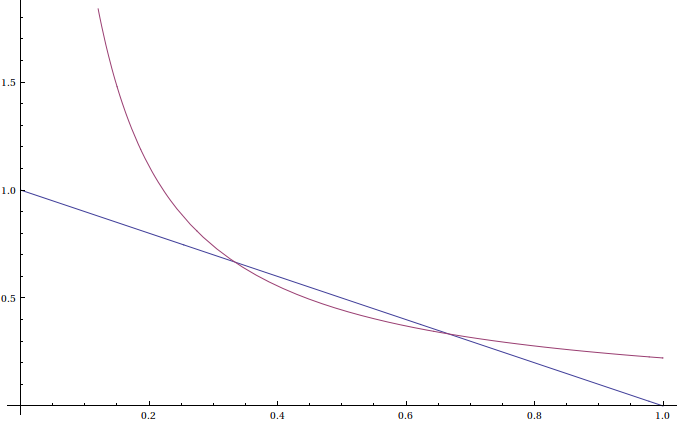
\includegraphics[width=\textwidth]{overlap.png}
\caption{The Desired Region}
\end{figure}
Where does this come from?
\begin{eqnarray}
	x_1 + x_2 \leq 1 \\ 
	x_2 \leq 1 - x_1
\end{eqnarray}
which is the straight line.
\begin{eqnarray}
	x_1x_2 \leq \frac{2}{9} \\ 
	x_2 \leq \frac{2}{9 x_1}
\end{eqnarray}
A little bit of algebra shows that these two lines intersect at $\frac{1}{3}$ and $\frac{2}{3}$ so the area underneath the straight line but not above the curved line is
\begin{eqnarray}
	A =\int_0^{\frac{1}{3}}(1-x)dx + \int_{\frac{1}{3}}^{\frac{2}{3}}\frac{2}{9x}dx + \int_{\frac{2}{3}}^{1}(1-x)dx \\ 
	= \frac{5}{18} + \int_{\frac{1}{3}}^{\frac{2}{3}}\frac{2}{9x}dx + \frac{1}{18} \\
	= \frac{1}{3} + \int_{\frac{1}{3}}^{\frac{2}{3}}\frac{2}{9x}dx \\ 
	= \frac{1}{3	} + \frac{2 \ln 2}{9} \approx 0.487366
\end{eqnarray}
And the answer is properly normalized since the initial probability distributions were unity (the box length is only 1).
\textbf{Answer  verified}


\subsection{}
%problem 4.9
As we showed in example number 4, $p_{\eta}$ is the convolution of $p_{\xi_1}$ and $p_{\xi_2}$.
\begin{eqnarray}
	p_{\eta}(y) = \int_{-\infty}^{\infty} p_{\xi_1}(y-x)p_{\xi_2}(x)dx
\end{eqnarray}
I think the integration will look more logical if we stick in Heaviside step-functions.
\begin{eqnarray}
	p_{\eta}(y) = \frac{1}{6} \int_{-\infty}^{\infty}e^{-\frac{y-x}{3}}e^{-\frac{x}{3}}H(y-x)H(x)dx
\end{eqnarray}
Clearly $x$ has to be greater than zero and $y$ must be greater than x, leading to the following limits of integration.
\begin{eqnarray}
	p_{\eta}(y) = \frac{1}{6} \int_{0}^{y}e^{-\frac{y-x}{3}}e^{-\frac{x}{3}}dx \\
	= e^{-\frac{y}{3}}\left(1- e^{-\frac{y}{6}}  \right)
\end{eqnarray}
Only when y is greater than zero!
\textbf{Answer verified}

\subsection{}
%problem 4.10
Due to the magic of addition, finding the probability distribution of $\xi_1 + \xi_2 + \xi_3$ is no different than the probability distribution of $(\xi_1 + \xi_2) + \xi_3$ but we already know what the probability distribtution of the parenthesized quantity is:
\begin{equation}
	p_{\xi_1 + \xi_2}(y) = \int_{-\infty}^{\infty} p_{\xi_1}(y-x)p_{\xi_2}(x)dx
\end{equation}
Therefore the total combination is
\begin{equation}
	p_{\xi_1 + \xi_2+ \xi_3}(z) = \int_{-\infty}^{\infty} p_{\xi_1 + \xi_2}(z-y)p_{\xi_3}(y)dx
\end{equation}
\begin{equation}
	p_{\xi_1 + \xi_2+ \xi_3}(z) = \int_{-\infty}^{\infty} \left[ \int_{-\infty}^{\infty} p_{\xi_1}(z-y-x)p_{\xi_2}(x)dx \right]p_{\xi_3}(y)dy
\end{equation}
\begin{equation}
	p_{\xi_1 + \xi_2+ \xi_3}(z) = \int_{-\infty}^{\infty}  \int_{-\infty}^{\infty} p_{\xi_1}(z-y-x)p_{\xi_2}(x)p_{\xi_3}(y)dx dy
\end{equation}
which is just a triple convolution.

\textbf{Answer not verified}

\subsection{}
%problem 4.11
\begin{equation}
	p_{\xi}(n) = \frac{1}{3^n}
\end{equation}
therefore
\begin{equation}
	\textbf{E}\xi = \sum_{n=1}^{\infty}\frac{n}{3^n} =  \frac{3}{4}
\label{answer4.11}
\end{equation}
\textbf{Answer not verified}

\subsection{}
%problem 4.12
Since finding a ball in one urn versus the other urn has nothing to do with each other, the events are clearly independent so we can multiply probabilities.  The probability of finding a white ball at any given urn is
\begin{equation}
	p_w = \frac{w}{w+b}
\end{equation}
If you find a white ball on the $n^{th}$ try then that means you found $n-1$ black balls before you got to the white ball.  
\begin{equation}
	p_w(n) = \frac{b^{n-1} w}{(w+b)^n}
\end{equation}
\begin{equation}
	\textbf{E}n = \sum_{i=1}^{\infty}n p_w(n) = \sum_{i=1}^{\infty}n \frac{b^{n-1} w}{(w+b)^n} = \frac{b+w}{w}
\end{equation}
Which is the total number of balls drawn, subtract one to get the average number of black balls drawn:
\begin{equation}
	m=\frac{b}{w}
\end{equation}
Now for the variance. to start with we need the average of the square of the random variable.
\begin{equation}
	\textbf{E}n^2 = \sum_{i=1}^{\infty}n^2 p_w(n) = \sum_{i=1}^{\infty}n^2 \frac{b^{n-1} w}{(w+b)^n} = \frac{(b+w) (2 b+w)}{w^2}
\end{equation}
\begin{equation}
	\textbf{D}n = \textbf{E}n^2 - (\textbf{E}n)^2 =  \frac{(b+w) (2 b+w)}{w^2} - \left( \frac{b+w}{w} \right)^2 = \frac{b^2+wb}{w^2}
\end{equation}
A note that we don't need to subtract anything for the variance since shifting a distribution over does not affect its variance: just its average.
\textbf{Answer verified}



\subsection{}
%problem 4.13
\begin{equation}
	\textbf{E}\xi = \int_{-\infty}^{\infty} x\frac{1}{2}e^{-|x|} = 0
\end{equation}
because the function is even about $x=0$.
\begin{equation}
	\textbf{E}\xi^2 = \int_{-\infty}^{\infty} x^2\frac{1}{2}e^{-|x|} = 2
\end{equation}
Therefore:
\begin{equation}
	\textbf{D}\xi = \textbf{E}\xi^2 - (\textbf{E}\xi)^2 = 2
\end{equation}
\textbf{Answer verified}




\subsection{}
%problem 4.14
\begin{equation}
	\textbf{E}x = \int_{a-b}^{a+b} \frac{xdx}{2b} = a	
\end{equation}
\begin{equation}
	\textbf{E}x^2 = \int_{a-b}^{a+b} \frac{x^2dx}{2b} = a^2+\frac{b^2}{3}
\end{equation}
Therefore:
\begin{equation}
	\textbf{D}x = \frac{b^2}{3}
\end{equation}
\textbf{Answer verified}


\subsection{}
%problem 4.15
If the distribution function is 
\begin{equation}
	\Phi_{\xi}(x) = a + b \arcsin x, |x| \leq 1
\end{equation}
then it must fulfill the proper boundary conditions as specified by both the problem and the definition of a distribution function.
\begin{equation}
	\Phi_{\xi}(-1)= 0 = a - b \frac{\pi}{2}
\end{equation}
\begin{equation}
	\Phi_{\xi}(1) = 1 = a + b \frac{\pi}{2}
\end{equation}
Some easy algebra gets you
\begin{eqnarray}
	\Phi_{\xi}(x) = \frac{1}{2} + \frac{1}{\pi} \arcsin x
\end{eqnarray}
Therefore:
\begin{equation}
	p_{\xi}(x) = \frac{1}{\pi\sqrt{1-x^2}}
\end{equation}
\begin{eqnarray}
	\textbf{E}x = \int_{-1}^{1} \frac{x dx}{\pi\sqrt{1-x^2}} = 0 \\
	\textbf{D}x = \int_{-1}^{1} \frac{x^2 dx}{\pi\sqrt{1-x^2}} = \frac{1}{2}
\end{eqnarray}
\textbf{Answer verified}



\subsection{}
%problem 4.16
Each side of the die has the same probability, $\frac{1}{6}$
\begin{equation}
	\textbf{E}x = \sum_{i=1}^6 \frac{i}{6} = \frac{7}{2}
\end{equation}
\begin{equation}
	\textbf{E}x^2 = \sum_{i=1}^6 \frac{i^2}{6} = \frac{91}{6}
\end{equation}
Therefore:
\begin{equation}
	\textbf{D}x = \frac{91}{6} - \left( \frac{7}{2} \right)^2 = \frac{91}{6} - \frac{49}{4} = \frac{35}{12}
\end{equation}
\textbf{Answer verified}

\subsection{}
%problem 4.17
This problem may seem difficult until you realize that being $\pm \frac{5}{2}$ away from the mean means you're at either 1 or 6, meaning that there's a unity probability of being that far from the mean.  Chebyshev's inequality, however, would have us believe that 
\begin{equation}
	P \{ |x + \textbf{E}x| > \frac{5}{2}  \} \leq \frac{4}{25} \frac{91}{6} = \frac{182}{75} = 2.42667
\end{equation}
which is not only far off from the actual answer, it's also unphysical to have probabilities greater than 1!
\textbf{Answer not verified}

\subsection{}
%problem 4.18
We want to consider the probability distribution of $\xi$ by way of $\eta$
\begin{equation}
	\eta = e^{\frac{a\xi}{2}} 
\end{equation}
We know from Chebyshev's identity:

\begin{equation}
	P\{ \eta > \epsilon(\eta) \} \leq \frac{\textbf{E}\eta^2}{\epsilon(\eta)^2} 
\end{equation}
Let $\epsilon$ be the error in $\xi$ we're looking for.
\begin{equation}
	P\{ \xi > \epsilon \} \leq \frac{\textbf{E}(e^{\frac{a\xi}{2}})^2}{(e^{\frac{a\epsilon}{2}})^2} 
\end{equation}
\begin{equation}
	P\{ \xi > \epsilon \} \leq \frac{\textbf{E}e^{a\xi}}{e^{a\epsilon}} 
\end{equation}
\textbf{Answer not verified}


\subsection{}
%problem 4.19
First some initial calculations:
\begin{eqnarray}
	\textbf{E}\xi = \frac{1}{4} \left( -2+-1+1+2  \right) = 0 \\
	\textbf{E}\xi^2 = \frac{1}{4} \left( (-2)^2+(-1)^2+1^2+2^2  \right) = \frac{10}{4} = \frac{5}{2} = \textbf{E}\eta \\
	\textbf{E}\xi^4 = \frac{1}{4} \left( (-2)^4+(-1)^4+1^4+2^4  \right) = \frac{34}{4} = \frac{17}{2} = \textbf{E}\eta^2
\end{eqnarray}
Now, we know that
\begin{eqnarray}
	r = \frac{\textbf{E} \left[ (\xi - \textbf{E}\xi)(\eta - \textbf{E}\eta)  \right]}{(\textbf{E}\xi^2 - (\textbf{E}\xi)^2)(\textbf{E}\eta^2 - (\textbf{E}\eta)^2)}
\end{eqnarray}
The denominator $D$ is the easiest:
\begin{equation}
	D = \left( \frac{5}{2} - 0 \right)\left( \frac{17}{2} - \frac{5^2}{2^2} \right) = \frac{45}{8}
\end{equation}
Now for the numerator:
\begin{eqnarray}
	\textbf{E} \left[ (\xi - \textbf{E}\xi)(\eta - \textbf{E}\eta)  \right] \\
	= \frac{1}{16} \left[  \sum_{\xi, \eta} (\xi - \textbf{E}\xi)(\eta - \textbf{E}\eta)      \right]
\end{eqnarray}
If we look at the set we'll be summing over, we have ${\xi - \textbf{E}\xi} = -2, -1, 1, 2$ and ${\eta - \textbf{E}\eta} = \frac{3}{2}, -\frac{3}{2}, -\frac{3}{2}, \frac{3}{2}$ and clearly, since we have to sum over all possible products, since both distributions are symmetric about 0, the sum will go to zero.
\begin{equation}
	r=0
\end{equation}
\textbf{Answer not verified}

\subsection{}
%problem 4.20
First some initial calculations:
\begin{eqnarray}
	\textbf{E}x_1 = \int_0^{\frac{\pi}{2}} x_1 \sin x_1 \sin x_2 dx_1dx_2 = 1 \\
	\textbf{E}x_2 = 1 \\
	\textbf{E}x_1^2 = \int_0^{\frac{\pi}{2}} x_1^2 \sin x_1 \sin x_2 dx_1dx_2 = (\pi - 2) \\
	\textbf{E}x_2^2 = (\pi - 2) \\
\end{eqnarray}
\begin{eqnarray}
	\textbf{E} \left[ (x_1 - \textbf{E}x_1)(x_2 - \textbf{E}x_2)  \right] \\
	= \int_0^{\frac{\pi}{2}} \int_0^{\frac{\pi}{2}} \left[(x_1 - 1)(x_2 - 1)\right]\sin x_1 \sin x_2 dx_1dx_2 = 0 \\
	\sigma_1 \sigma_2 =  \sqrt{(\pi - 2)- 1}\sqrt{(\pi - 2) - 1} = (\pi - 3) \\
	r= \frac{0}{(\pi - 3)} = 0
\end{eqnarray}
\textbf{Answer not verified}

\subsection{}
%problem 4.21
First some initial calculations:
\begin{eqnarray}
	\textbf{E}x_1 = \frac{1}{2}\int_0^{\frac{\pi}{2}} x_1 \sin (x_1 + x_2) dx_1dx_2 = \frac{\pi}{4} \\
	\textbf{E}x_2 = \frac{\pi}{4} \\
	\textbf{E}x_1^2 = \frac{1}{2}\int_0^{\frac{\pi}{2}} x_1^2 \sin (x_1 + x_2) dx_1dx_2 = -2+\frac{\pi}{2} +\frac{\pi ^2}{8} \\
	\textbf{E}x_2^2 = -2+\frac{\pi}{2} +\frac{\pi ^2}{8} \\
\end{eqnarray}
\begin{eqnarray}
	\textbf{E} \left[ (x_1 - \textbf{E}x_1)(x_2 - \textbf{E}x_2)  \right] \\
	= \frac{1}{2}\int_0^{\frac{\pi}{2}} \int_0^{\frac{\pi}{2}} \sin (x_1 + x_2) \left[(x_1 - \frac{\pi}{2})(x_2 - \frac{\pi}{2})\right]dx_1dx_2  = -\frac{1}{16} (\pi -4)^2 \\
	\sigma_1\sigma_2 = -2+\pi +\frac{\pi ^2}{2} +\frac{\pi^2}{8} - \frac{\pi^2}{16} = -2+\pi +\frac{\pi ^2}{2} +\frac{\pi^2}{16} \\
	r = \frac{-\frac{1}{16} (\pi -4)^2}{-2+\pi +\frac{\pi ^2}{2} +\frac{\pi^2}{16}}
\end{eqnarray}
\textbf{Answer verified}

\subsection{}
%problem 4.22
Ill-defined problem, don't feel like translating: \textbf{SKIPPED}

\subsection{}
%problem 4.23
Based off 4.22: \textbf{SKIPPED}

\subsection{}
%problem 4.21
\begin{eqnarray}
	E\xi = \int_{-\infty}^{\infty} \frac{x}{\pi(1+x^2)}dx = \left \frac{\log \left(x^2+1\right)}{2 \pi } \right]_{-\infty}^{\infty} \rightarrow \infty \\
	E\xi^2 = \int_{-\infty}^{\infty} \frac{x^2}{\pi(1+x^2)}dx = \left \frac{x}{\pi }-\frac{\tan ^{-1}(x)}{\pi } \right]_{-\infty}^{\infty} \rightarrow \infty
\end{eqnarray}
Neither integral actually converges so we cannot define averages or dispersions for this distribution.
\textbf{Answer verified}
%%answer template
%\subsection{}
%%problem n.n
%
%
%\begin{equation}
%	
%\label{answern.n}
%\end{equation}
%\textbf{Answer [not] verified}








\chapter{Three Important Probability Distributions}

\section{Important/Useful Theorems}

\subsection{The Binomial Distribution}
For $n$ trials where the probability of success is $p$ and the probability of failure is $q=1-p$, the probability of their being $k$ successes is:
\begin{equation}
	p(k) = \binom{n}{k} p^k q^{n-k}
\end{equation}

\subsection{The Poisson Distribution}
For $n$ trials where the probability of success is $p$ and is very small and the number of trials is very large, the probability of their being $k$ successes is:
\begin{equation}
	p(k) = \frac{a^k}{k!}e^{-a}
\end{equation}
Where $a=np$, the average number of successes.

\subsection{The Normal Distribution}
As $n \rightarrow \infty$, the Binomial Distribution goes to:
\begin{equation}
	p(x) = \frac{1}{\sqrt{2 \piu \sigma^2}}e^{\frac{-(x-a)^2}{2 \sigma^2}}
\end{equation}


\section{Answers to Problems}


\subsection{}
%problem5.1
If you call tails, there are two possibilities for the outcome of the coin-toss experiment which, since they are not correlated to your guess, are both one-half; similarly for heads.  Therefore, no matter what you do, the probability of guessing correctly is one-half.

If, however, the coin is biased towards heads, there is a probability greater than one half that you'll win the trial if you call heads; therefore you should always call heads for a coin biased towards heads and similarly always call tails for a coin biased towards tails.

\end{equation}
\textbf{Answer not verified}


\subsection{}
%problem5.2

In order to avoid any blatant sexism, we shall define  ``success'' as having a boy... What?  Anyway, for a couple having $n$ children, the probability of having $k$ boys will clearly follow a binomial distribution:

\begin{equation}
	p_n(k) = \binom{n}{k} \frac{1}{2^n}
\end{equation}
\subsubsection{a}
\begin{equation}
	p_{10}(5) = \binom{10}{5} \frac{1}{2^{10}} = \frac{63}{256} = 0.246094
\end{equation}
\subsubsection{b}
\begin{equation}
	p_{10}(3\rightarrow 7) = \sum_{i = 3}^7 \binom{10}{i} \frac{1}{2^{10}} = \frac{57}{64} = 0.890625
\end{equation}
\textbf{Answer not verified}


\subsection{}
%problem5.3

Since $p=.001$ and $n=5000$ we can cautiously use the Poisson Distribution where $a=5$.  Since we want to know the probability of hitting 2 or more, we will take the probability of hitting either 0 or 1 and subtract from 1.

\begin{equation}
	p(k \geq 2) = 1 - p(0) - p(1) \approx 1 - \frac{5^0}{0!}e^{-5} - \frac{5^1}{1!}e^{-5} = 1 - 6e^{-5} \approx 0.96
\end{equation}

\textbf{Answer verified}

\subsection{}
%problem5.4

Again we cautiously use the Poisson Distribution since $p=\frac{1}{500}$ and $n=500$ and again use the same trick as before to get the chance of greater than two ``successes''.
\begin{equation}
	p(k \geq 2) = 1 - p(0) - p(1) \approx 1 - \frac{1^0}{0!}e^{-1} - \frac{1^1}{1!}e^{-1} = 1 - \frac{2}{e} \approx 0.264241
\end{equation}
Note that the book has most definitely got this problem wrong as:
\begin{equation}
	p(k \geq 3) = 1 - p(0) - p(1) - p(2) \approx 1 - \frac{1^0}{0!}e^{-1} - \frac{1^1}{1!}e^{-1}- \frac{1^2}{2!}e^{-1} = 1 - \frac{5}{2e} \approx .0803
\end{equation}

\textbf{Answer verified-ish}


\subsection{}
%problem5.5

Without any special cases, this problem is the good-old binomial distribution:

\begin{equation}
	p(k) = \binom{n}{k} p^k(1-p)^{n-k}
\end{equation}
So we simply sum up all the even probabilities:
\begin{equation}
	P_n = \sum_{i=0}^{\frac{n}{2}} p(2i) = \sum_{i=0}^{\frac{n}{2}} \binom{n}{2i} p^{2i}(1-p)^{2i-k}
\end{equation}
Which in the total lack of any skill in mathematics, I plug into Mathematica to get:
\begin{equation}
	P_n = \frac{1}{2} \left((1-2 p)^n+1\right)
\end{equation}

\textbf{Answer verified}

\subsection{}
%problem5.6
In an infinite series of Bernouli trials, let the event that the $i^{th}$ 3-tuple has the pattern SFS be $A_i$ and $P(A_i)=p_i$.  Since we've designed these tuples to not overlap, these trials are independent such that:
\begin{equation}
	P\left( \bigcup_{i=1}^{\infty} A_i \right) = \sum _{i=1}^{\infty} p_i \rightarrow \infty
\end{equation}
By the second Borel-Cantelli lemma.

\textbf{Answer not verified}

\subsection{}
%problem5.7

WE want the probability of 3 or more very rare events happening in a large number of trials: this is a Poisson distribution with $a=1000\cdot0.001=1$
\begin{equation}
	p(k \geq 3) = 1 - p(0) - p(1) - p(2) \approx 1 - \frac{1^0}{0!}e^{-1} - \frac{1^1}{1!}e^{-1}- \frac{1^2}{2!}e^{-1} = 1 - \frac{5}{2e} \approx .0803
\end{equation}

\textbf{Answer not verified}

\subsection{}
%problem5.8

We'll go ahead and call $p=\frac{1}{365}$ to be small and 730 to be big so that we can do Poisson with $a=2$.
\begin{equation}
	p(2) = \frac{2^2}{2!}e^{-2} = \frac{2}{e^2} \approx 0.270671
\end{equation}

\textbf{Answer not verified}

\subsection{}
%problem5.9

\begin{equation}
	\textbf{E}\xi = \sum_{k=0}^{\infty} k \frac{a^k}{k!}e^{-a} = e^{-a}a\sum_{k=0}^{\infty} \frac{a^{(k-1)}}{(k-1)!} = a
\end{equation}
\begin{equation}
	\textbf{E}\xi^2 = \sum_{k=0}^{\infty} k^2 \frac{a^k}{k!}e^{-a} = a^2 + a
\end{equation}
That last one I got lazy and used Mathematica, sorry!  Clearly, though $\sigma^2 = a$.
\begin{eqnarray}
	\frac{\textbf{E}(\xi - a)^3}{\sigma^3} = \frac{\textbf{E}(\xi^3 - 3\xi^2a + 3\xia^2 - a^3)}{a^{\frac{3}{2}}} \\
	 \textbf{E}\xi^3 = a^3+3 a^2+a \\
	 \textbf{E}(\xi^3 - 3\xi^2a + 3\xi a^2 - a^3) = (a^3+3 a^2+a) - 3a(a^2 + a) + 3a^3 - a^3 = a \\
	 \frac{\textbf{E}(\xi - a)^3}{\sigma^3} = \frac{a}{a^{\frac{3}{2}}} = \frac{1}{\sqrt{a}}
\end{eqnarray}
\textbf{Answer verified}

\subsection{}
%problem5.10

\textbf{SKIPPED}

\subsection{}
%problem5.11
Finally! something other than the Poisson distribution... back to... NORMAL!  Ha!
\begin{eqnarray}
	\textbf{E}x = np = 30 \\
	\textbf{D}x = npq = 30\cdot .7 = 21 \\
	p = \int_{20}^{40} \frac{1}{\sqrt{2 \pi 21}} e^{\frac{-(x-30)^2}{2 \cdot 21}} \approx 0.970904
\end{eqnarray}
\textbf{Answer verified}


\subsection{}
%problem5.12
We want to know at one $n$ does this integral
\begin{eqnarray}
	\int_{.3}^{.5} \frac{1}{\sqrt{2 \pi .24/n}} e^{\frac{-(x-.4)^2}{2 \cdot .24/n}} \approx 0.9
\end{eqnarray}
A first pass going at intervals of 10 identifies the number being between 60 and 70 and a further pass going by one reveals that going from 64 to 65 breaks the .89 barrier.  Therefore $n=65$.

Note that in order to get that $n$ in the denominator, we are taking the relative mean and the relative standard deviation: since both quantities get divided by $n$, the square of the standard deviation ends up with an $n$ in the denominator.
\textbf{Answer verified}

\subsection{}
%problem5.13

\begin{eqnarray}
	\textbf{E}x = 60 \cdot .6 = 36 \\
	\textbf{D}x = 36 \cdot .4 = 14.4 \\
	p = \int_{30}^{\infty} \frac{1}{\sqrt{2 \pi 14.5}} e^{\frac{-(x-36)^2}{2 \cdot 14.4}} \approx 0.943077
\end{eqnarray}

\textbf{Answer verified}

\subsection{}
%problem5.14
Perform the integrals as suggested.  Why can you?  Well, it feels right, doesn't it?  I found it impossible to come up with other than an intuitive reason for why this is true: sorry dear reader.

\textbf{Answer verified-ish}

\subsection{}
%problem5.15

\textbf{SKIPPED}


\subsection{}
%problem5.16
Convolute the two distributions and the intended expression will come out: BOM!

\textbf{Answer verified-ish}

%%answer template
%\subsection{}
%%problem n.n
%
%
%\begin{equation}
%	
%\label{answern.n}
%\end{equation}
%\textbf{Answer [not] verified}








\chapter{Some Limit Theorems}

\section{Important/Useful Theorems}

\subsection{Weak Law of Large Numbers}
Let $\xi_1, \xi_2, ..., \xi_n$ be $n$ independent indentically distributed random variables with mean $a$ and variance $\sigma^2$.  Then, given any $\delta > 0$ and $\epsilon >0$, however small, there is an integer, $n$ such that:
\begin{equation}
	a- \epsilon \leq \frac{1}{n}(\xi_1 +\xi_2 + \cdots + \xi_n) \leq a + \epsilon
\end{equation}
with probability greater than $1- \delta$.


\subsection{Generating Functions}

For the \textbf{discrete} random variable $\xi$ with probability distribution $P_{\xi}(k)$, the generating function is defined as

\begin{equation}
	F_{\xi}(z) = \sum_{k=0}^{\infty}P_{\xi}(k)z^k
\end{equation}
which yields some cool relations:
\begin{eqnarray}
	P_{\xi}(k) = \frac{1}{k!}F_{\xi}^{(k)}(0) \\
	\textbf{E}\xi = F'(1) \\
	\sigma^2 =F''(1) + F'(1) - [F'(1)]^2
\end{eqnarray}

Note, also, that while you sum together random variables, you multiply generating functions.

\subsection{Thm. 6.2}

The sequence of probability distributions, $P_n(k)$ with generating functions $F_n(z)$ where $n=1, 2, 3, ....$ converges weakly to the distribution $P(k)$ with distribution function $F(z)$ iff  

\begin{equation}
	\lim_{n\rightarrow \infty} F_n(z) = F(z)
\end{equation}

\subsection{Characteristic Functions}

For a real random variable $\xi$, its generating function is defined as

\begin{equation}
	f_{\xi}(t) = \textbf{E}e^{i \xi t} = F_{\xi}(e^{i t}) = \sum_{k=0}^{\infty} P_{\xi}(k)e^{i k t}
\end{equation}
Or, if the variable is continuous:
\begin{equation}
	f_{\xi}(t) = \int_{-\infty}^{\infty} P_{\xi}(x)e^{i x t} dx
\end{equation}
Where it is clear that is represents the discrete or continuous fourier transform of the probability distribution and as such, the inverse is true:
\begin{equation}
	P_{\xi}(x) = \frac{1}{2 \pi}\int_{-\infty}^{\infty} f_{\xi}(t)e^{-i x t} dt
\end{equation}
Like Generating functions, there are some cool properties that can be exploited:
\begin{eqnarray}
	\textbf{E}\xi = -if_{\xi}'(0) \\
	\textbf{D}\xi = -f_{\xi}''(0) + [f_{\xi}'(0)]^2
\end{eqnarray}
And just like generating functions, they multiply together for random variables that add together.

\subsection{The Central Limit Theorem}

A sequence of random variables $\xi_1, \xi_2, \xi_3, ...$ is said to satisfy the central limit theorem if
\begin{equation}
	\lim_{n\rightarrow \infty} \textbf{P}\{ x' \leq \frac{S_n - \textbf{E}S_n}{\sqrt{\textbf{D}S_n}} \leq x''\} = \int_{x'}^{x''}e^{\frac{-x^2}{2}}dx
\end{equation}
Where
\begin{equation}
	S_n = \sum_{k=1}^n \xi_k
\end{equation}

\subsection{Thm. 6.3}

If the same series of random variables as above each has mean $a_k$ and variance $\sigma^2_k$ and satisfies the Lyapunov condition:
\begin{equation}
	\lim_{n\rightarrow \infty} \frac{1}{B_n^3} \sum_{k=1}^n \textbf{E}|\xi_k - a_k|^3 = 0
\end{equation}
Where
\begin{equation}
	B_n^2 = \textbf{D}S_n = \sum_{k=1}^n \sigma^2_k
\end{equation}
then the sequence will satisfy the central limit theorem.


\section{Answers to Problems}
\subsection{}
%problem6.1
\begin{eqnarray}
	a- \epsilon \leq \frac{1}{n}(\xi_1 +\xi_2 + \cdots + \xi_n) \leq a + \epsilon \\
	a- \epsilon \leq \frac{1}{n}\sum_{k=1}^n \xi_i \leq a + \epsilon \\
	- \epsilon \leq \frac{1}{n}\sum_{k=1}^n \xi_i -a \leq \epsilon \\
	\left| \frac{1}{n}\sum_{k=1}^n \xi_i -a  \right| < \epsilon
\end{eqnarray}
And we know this happens with probability
\begin{equation}
	P_n = 1- \delta
\end{equation}
\begin{equation}
	\textbf{P} \left[ \left| \frac{1}{n}\sum_{k=1}^n \xi_i -a  \right| < \epsilon  \right] = 1 - \delta
\end{equation}
\begin{equation}
	\lim_{n\rightarrow \infty} \textbf{P} \left[ \left| \frac{1}{n}\sum_{k=1}^n \xi_i -a  \right| < \epsilon  \right] = 1 
\end{equation}
\textbf{Answer not verified}

\subsection{}
%problem6.2

Since we know the mean, we most certainly can use the equation to estimate the variance: look what it's doing.  It's taking the sum of the square of the distances from the known mean and dividing by the number of trials: the classic standard deviation calculation.
\textbf{Answer not verified}

\subsection{}
%problem6.3
We need to start with some calculations on the distribution:
\begin{eqnarray}
	E\xi = \int_0^{\infty} x \frac{x^m}{m!}e^{-x} dx = m+1 \\
	E\xi^2 = \int_0^{\infty} x^2 \frac{x^m}{m!}e^{-x} dx = (m+2)(m+1)
\end{eqnarray}

\begin{equation}
	P \{  | \xi - a | > \epsilon  \} \leq \frac{1}{\epsilon^2}\textbf{E}(\xi - a)^2
\end{equation}
clearly we can manipulate it in this manner:
\begin{equation}
	-P \{  | \xi - a | > \epsilon  \} \geq  - \frac{1}{\epsilon^2}\textbf{E}(\xi - a)^2
\end{equation}
\begin{equation}
	1-P \{  | \xi - a | > \epsilon  \} \geq 1 - \frac{1}{\epsilon^2}\textbf{E}(\xi - a)^2
\end{equation}
\begin{equation}
	P \{  | \xi - a | < \epsilon  \} \geq 1 - \frac{1}{\epsilon^2}\textbf{E}(\xi - a)^2
\end{equation}
let $\epsilon = a = m+1$
\begin{equation}
	P \{ 0 \leq \xi  \leq 2(m+1)  \} \leq 1 - \frac{1}{(m+1)^2}[(m+2)(m+1) - (m+1)^2]
\end{equation}
\begin{equation}
	P \{ 0 \leq \xi  \leq 2(m+1)  \} \leq \frac{m}{m+1}
\end{equation}

\textbf{Answer not verified}

\subsection{}
%problem6.4
Under these circumstances, we expect 500 A and the standard deviation is $\sqrt{250}= 5 \sqrt{10} \approx 15$ therefore the $\pm 100$ from the mean is more than $\pm 6 \sigma$ meaning there is indeed far more that .97 probability of seeing the mean between these two values.


\textbf{Answer not verified}


\subsection{}
%problem6.5
\begin{eqnarray}
	F_{\xi}(z) = \frac{z +z^2 + z^3 + z^4 + z^5 +z^6}{6}
\end{eqnarray}

\textbf{Answer not verified}

\subsection{}
%problem6.6
\begin{eqnarray}
	F'_{\xi}(z) = \frac{1+ 2z + 3z^2 + 4z^3 + 5z^4 + 6z^5}{6}
\end{eqnarray}
\begin{eqnarray}
	F'_{\xi}(1) = \frac{21}{6} = \frac{7}{2} = \textbf{E}\xi
\end{eqnarray}
\begin{eqnarray}
	F''_{\xi}(z) = \frac{2+ 6z + 12z^2 + 20z^3 + 30z^4 }{6}
\end{eqnarray}
\begin{eqnarray}
	F''_{\xi}(1) = \frac{70}{6} = \frac{35}{3}  
\end{eqnarray}
\begin{eqnarray}
	\sigma^2 = F''_{\xi}(1) + F'_{\xi}(1) + [F'_{\xi}(1)]^2  = \frac{35}{3} + \frac{7}{2} - \frac{49}{4}  = \frac{35}{12}
\end{eqnarray}
\textbf{Answer verified}

\subsection{}
%problem6.7
In order to do this problem with 6.6, we need the generating function
\begin{eqnarray}
	F_{\xi}(z) = \sum_{k=0}^{\infty} \frac{ a^k }{k!}e^{-a} z^k = e^{a(z-1)}
\end{eqnarray}
\begin{eqnarray}
	F'_{\xi}(z) = a e^{a (z-1)} \\
	F'_{\xi}(1) = a e^{0}  = a = \textbf{E}\xi\\
\end{eqnarray}
\begin{eqnarray}
	F''_{\xi}(z) = a^2 e^{a (z-1)} \\
	F''_{\xi}(1) = a^2
\end{eqnarray}
\begin{eqnarray}
	\sigma^2 = F''_{\xi}(1) + F'_{\xi}(1) - [F'_{\xi}(1)]^2  = a^2 + a - a^2 = a
\end{eqnarray}


\subsection{}
%problem6.8
In order to do this problem with 6.6, we need the generating function
\begin{eqnarray}
	F_{\xi}(z) = \sum_{k=0}^{\infty} \frac{ a^k }{(1+a)^{k+1}} z^k = \frac{-a-1}{(a+1) (a z-a-1)}
\end{eqnarray}
\begin{eqnarray}
	F'_{\xi}(z) = \frac{(a+1) a}{(a+1) (a z-a-1)^2} = \frac{a}{(a z-a-1)^2} \\
	F'_{\xi}(1) = a =  \textbf{E}\xi\\
\end{eqnarray}
\begin{eqnarray}
	F''_{\xi}(z) = \frac{-2 a^2}{(a z-a-1)^3} \\
	F''_{\xi}(1) = 2 a^2
\end{eqnarray}
\begin{eqnarray}
	\sigma^2 = F''_{\xi}(1) + F'_{\xi}(1) - [F'_{\xi}(1)]^2  = 2 a^2 + a - a^2 = a^2 - a = \textbf{D}\xi
\end{eqnarray}

\textbf{Answer not verified}


\subsection{}
%problem6.9
These two distributions have generating functions:
\begin{eqnarray}
	F_{\xi_1} = e^{a(z-1)} \\
	F_{\xi_2} = e^{a'(z-1)}
\end{eqnarray}
which means that $\eta$ has this generating function:
\begin{eqnarray}
	F_{\eta} =F_{\xi_1}F_{\xi_2} = e^{a(z-1)}e^{a'(z-1)} = e^{(a'+ a)(z-1)}  \\
\end{eqnarray}
Which, according to theorem 6.2 means there that $\eta$ is a Poisson distribution with mean $a+a'$.
\textbf{Answer not verified}


\subsection{}
%problem6.10
For any given experiment we can define an individual generating function: $F_i(z) = q_i + z p_i$ meaning that for the entire function
\begin{eqnarray}
	F(z) = \prod_{i=1}^n F_i(z) = \prod_{i=1}^n (q_i + z p_i)
\end{eqnarray}
The trick that Feller uses at this point is to take the log
\begin{eqnarray}
	\log F(z) = \sum_{i=1}^n \log F_i(z) = \sum_{i=1}^n \log (q_i + z p_i) \\
	\log F(z) = \sum_{i=1}^n \log (1 - p_i + z p_i) = \sum_{i=1}^n \log (1 - p_i( z -1))
\end{eqnarray}
We were, however, told that the largest probability goes to zero so we take the taylor series of each term, $\log (1-x) \approx - x$
\begin{eqnarray}
	\lim_{n \rightarrow \infty} \log F(z) =  \sum_{i=1}^n \log (1 - p_i( z -1)) = \sum_{i=1}^n  p_i( 1 - z ) = - \lambda (z - 1) \\
	\lim_{n \rightarrow \infty} F(z) = e^{- \lambda (z - 1)}
\end{eqnarray}
And, according to theorem 6.2, the probability distribution is Poissonian.
\textbf{Answer verified}


\subsection{}
%problem6.11

\begin{eqnarray}
	p_{\xi}(x) = \frac{1}{2} e^{-|x|} \\
	f_{\xi}(t) = \int_{-\infty}^{\infty} \frac{1}{2} e^{ i x t } e^{-|x|} dx \\
	f_{\xi}(t) = \frac{1}{t^2+1}
\end{eqnarray}

\textbf{Answer verified}

\subsection{}
%problem6.12
\begin{eqnarray}
	f_{\xi}(t) = \frac{1}{t^2+1} \\
	f'_{\xi}(t) =  -\frac{2 t}{\left(t^2+1\right)^2} = i \textbf{E}\xi \\
	f'_{\xi}(0) =  i \textbf{E}\xi = 0 \\
	f''_{\xi}(t) = \frac{8 t^2}{\left(t^2+1\right)^3}-\frac{2}{\left(t^2+1\right)^2} \\
	f''_{\xi}(0) = - \sigma^2 = -2
\end{eqnarray}

\textbf{Answer verified}


\subsection{}
%problem6.13
For a uniform distribution
\begin{eqnarray}
	p(x) = \frac{1}{b-a}
\end{eqnarray}
Therefore the characteristic is:
For a uniform distribution
\begin{eqnarray}
	f(t) = \frac{1}{b-a} \int_a^b e^{i x t} dx = \frac{i \left(e^{i a t}-e^{i b t}\right)}{t(b-a)}
\end{eqnarray}
\textbf{Answer verified}


\subsection{}
%problem6.14
\begin{eqnarray}
	f_{\xi} (t) = e^{-a|t|} \\
	p(x) = \frac{1}{2 \pi} \inf_{\infty}^{\infty} e^{-a|t|} e^{- i x t} \\
	p(x) = \frac{a}{\pi(a^2+x^2)}
\end{eqnarray} 
\textbf{Answer verified}

\subsection{}
%problem6.15
Looking at the characteristic, there is clearly going to be a discontinuity in the deirvative at $t=0$, meaning that the derivative does not exist at that point.  This jibes well with what we've done before because we proved in problem 43 on page 24 that the probability distribution this characteristic produces does not have a mean or a standard deviation.

\textbf{Answer not verified}


\subsection{}
%problem6.16
For the single die, $E\xi = 3.5$ and $D\xi = \frac{35}{12}$.  The distribution for $n$ dice rolls is binomial but in the limit of large $n$, it approximates a normal distribution with $E\xi = 3.5n$ and $D\xi = n \frac{35}{12}$
\begin{eqnarray}
	P\{ 3450 \leq x \leq 3550  \} = \int_{3450}^{3550} \sqrt{\frac{1}{\frac{70 \pi \cdot 10^3}{12}}}e^{-\frac{(x-3500)^2}{\frac{70 \cdot 10^3}{12}}} dx \\
	= 0.645461  \\
\end{eqnarray} 
\textbf{Answer not verified}

\subsection{}
%problem6.17

We want to prove here that the distribution satisfies the Lyapunov condition:
\begin{equation}
	\lim_{n\rightarrow \infty} \frac{1}{B_n^3} \sum_{k=1}^n \textbf{E}|\xi_k - a_k|^3 = 0
\end{equation}
Where
\begin{equation}
	B_n^2 = \textbf{D}S_n = \sum_{k=1}^n \sigma^2_k
\end{equation}

The machinations of which are left to the reader... sorry!

\textbf{Answer not verified}

%%answer template
%\subsection{}
%%problem n.n
%
%
%\begin{equation}
%	
%\label{answern.n}
%\end{equation}
%\textbf{Answer [not] verified}








\chapter{Markov Chains}

\section{Important/Useful Theorems}

\subsection{}
For a Markox transition matrix, the limiting probabilities of being in a certain state as $n \rightarrow \infty$ are given by the solution to the following set of linear equations.
\begin{equation}
	p_j^* = \sum_{i=1}^{\infty} p_i^* p_{ij}
\end{equation}

\section{Answers to Problems}
\subsection{}
%problem 7.1
Since state $i$ signifies that the highest number chosen so far is $i$, what is the probability the next number is lower than $i$ and you stay in state $i$?  Well, there are $m$ possible numbers that could get picked and $i$ of them are less than or equal to $i$ giving:

\begin{equation}
	p_{ii} = \frac{i}{m}
\end{equation}

What now if we're in $i$ and we want to know what the probability of being in state $j$ is next.  Well, if $j<i$ then it's zero because you can't go to a lower number in this game.  If, however, $j$ is not lower then there are $m$ possible numbers that could get called and only one of them is $j$, giving:
\begin{equation}
	p_{ij} = \frac{1}{m}, j>i
\end{equation}
\begin{equation}
	p_{ij} = 0, j<i
\end{equation}

\textbf{Answer verified}

\subsection{}
%problem 7.2
Since the chain has an inevitable endpoint that you cannot get out of, there is a persistent state at $i=m$ while all other states are transient.  Transient, in that you will only see them a few times but $m$ is bound to show up sooner or later and once you're in $m$ you can't get out no matter what.

\textbf{Answer not verified}

\subsection{}
%problem 7.3
To do this properly we need to first construct the matrix $P$.
\begin{equation}
P = \left(
\begin{array}{ccccc}
 0 & \frac{1}{4} & \frac{1}{4} & \frac{1}{4} & \frac{1}{4} \\
 0 & \frac{1}{4} & \frac{1}{4} & \frac{1}{4} & \frac{1}{4} \\
 0 & 0 & \frac{1}{2} & \frac{1}{4} & \frac{1}{4} \\
 0 & 0 & 0 & \frac{3}{4} & \frac{1}{4} \\
 0 & 0 & 0 & 0 & 1
\end{array}
\right)
\end{equation}
Then we square it:
\begin{equation}
P^2 = 
\left(
\begin{array}{ccccc}
 0 & \frac{1}{16} & \frac{3}{16} & \frac{5}{16} & \frac{7}{16} \\
 0 & \frac{1}{16} & \frac{3}{16} & \frac{5}{16} & \frac{7}{16} \\
 0 & 0 & \frac{1}{4} & \frac{5}{16} & \frac{7}{16} \\
 0 & 0 & 0 & \frac{9}{16} & \frac{7}{16} \\
 0 & 0 & 0 & 0 & 1
\end{array}
\right)\end{equation}
\textbf{Answer not verified}


\subsection{}
%problem 7.4
So, if we start with $i$ balls in the urn, what is the probability that we have $j$ after drawing $m$ and discarding all the white balls.  The obvious first simplification we can make is that you can't end up with fewer that the $N-m$ white balls after drawing:
\begin{equation}
	p_{ij} = 0, j > N - m
\end{equation}
You also can't gain white balls
\begin{equation}
	p_{ij} = 0, j > i 
\end{equation}
OK! now for the interesting one.  There are $\binom{N}{m}$ ways to draw $m$ balls from the urn.  In any given step, you are going to draw $i-j$ white balls from a total of $i$ and $m - i +j$ black balls from a total of $N-i$.  Thus there are $\binom{i}{i-j}\binom{N-i}{m - i +j}$ ways to make that draw.
\begin{equation}
	p_{ij} = \frac{\binom{i}{i-j}\binom{N-i}{m - i +j}}{\binom{N}{m}}, \text{otherwise}
\end{equation}
\textbf{Answer verified}

\subsection{}
%problem 7.5
Once again, we start building the transition matrix.
\begin{equation}
	P = \left(
\begin{array}{ccccccccc}
 1 & 0 & 0 & 0 & 0 & 0 & 0 & 0 & 0 \\
 \frac{1}{2} & \frac{1}{2} & 0 & 0 & 0 & 0 & 0 & 0 & 0 \\
 \frac{3}{14} & \frac{4}{7} & \frac{3}{14} & 0 & 0 & 0 & 0 & 0 & 0 \\
 \frac{1}{14} & \frac{3}{7} & \frac{3}{7} & \frac{1}{14} & 0 & 0 & 0 & 0 & 0 \\
 \frac{1}{70} & \frac{8}{35} & \frac{18}{35} & \frac{8}{35} & \frac{1}{70} & 0 & 0 & 0 & 0 \\
 0 & \frac{1}{14} & \frac{3}{7} & \frac{3}{7} & \frac{1}{14} & 0 & 0 & 0 & 0 \\
 0 & 0 & \frac{3}{14} & \frac{4}{7} & \frac{3}{14} & 0 & 0 & 0 & 0 \\
 0 & 0 & 0 & \frac{1}{2} & \frac{1}{2} & 0 & 0 & 0 & 0 \\
 0 & 0 & 0 & 0 & 1 & 0 & 0 & 0 & 0
\end{array}
\right)

\end{equation}
And then just square it!
\begin{equation}
	P^2 = \left(
\begin{array}{ccccccccc}
 1 & 0 & 0 & 0 & 0 & 0 & 0 & 0 & 0 \\
 \frac{3}{4} & \frac{1}{4} & 0 & 0 & 0 & 0 & 0 & 0 & 0 \\
 \frac{107}{196} & \frac{20}{49} & \frac{9}{196} & 0 & 0 & 0 & 0 & 0 & 0 \\
 \frac{75}{196} & \frac{24}{49} & \frac{6}{49} & \frac{1}{196} & 0 & 0 & 0 & 0 & 0 \\
 \frac{1251}{4900} & \frac{624}{1225} & \frac{264}{1225} & \frac{24}{1225} & \frac{1}{4900} & 0 & 0 & 0 & 0 \\
 \frac{39}{245} & \frac{471}{980} & \frac{153}{490} & \frac{23}{490} & \frac{1}{980} & 0 & 0 & 0 & 0 \\
 \frac{22}{245} & \frac{102}{245} & \frac{393}{980} & \frac{22}{245} & \frac{3}{980} & 0 & 0 & 0 & 0 \\
 \frac{3}{70} & \frac{23}{70} & \frac{33}{70} & \frac{3}{20} & \frac{1}{140} & 0 & 0 & 0 & 0 \\
 \frac{1}{70} & \frac{8}{35} & \frac{18}{35} & \frac{8}{35} & \frac{1}{70} & 0 & 0 & 0 & 0
\end{array}
\right)
\end{equation}
Telling us there is a 39 in 245 chance that if we start with 5 balls that we'll be at zero after two steps.
\textbf{Answer verified}

\subsection{}
%problem 7.6
Since our chain is finite-dimensional and each state is accessible from every other state, all states are persistent by the corollary to theorem 7.3.

\textbf{Answer not verified}

\subsection{}
%problem 7.7
As the problem alludes to, if you start off on at any given point, there is zero probability of being at that point during the next step.  Hence, the elements of the transfer matrix oscillate between being 0 and non-zero so the limit of 7.20 is always zero and not greater than zero as implied.

\textbf{Answer not verified}


\subsection{}
%problem 7.8

Because you can now conceivably stay at the edge point, that means that every point is now accessible from every other point at every time step after a certain period of time has elapsed.  Since we're also finite dimensional and now accessible, 7.20 is now satisfied and we have proven the existence of the stationary probabilities.

\textbf{Answer not verified}

\subsection{}
%problem 7.9

We now want to solve:

\begin{equation}
	p_j^* = \sum_{i=1}^{m} p_i^* p_{ij}
\end{equation}
So let's get to it!

\begin{eqnarray}
	p_1^* = \sum_{i=1}^{m} p_i^* p_{i1} = q p_1^* + q p_2^* \\
	p_2^* = \sum_{i=1}^{m} p_i^* p_{i2} = p p_1^* + q p_3^* \\
	p_j^* = p p_{j-1}^* + q p_{j+1}^* \\
	p_m^* = \sum_{i=1}^{m} p_i^* p_{im} = p p_{m-1}^* + p p_{m}^*
\end{eqnarray}
You can easily solve the first equation to get:
\begin{equation}
	p_2^* =\frac{p}{q} p_1^*
\end{equation}
Then if we look to solve the second equation for $p_2^*$, 
\begin{eqnarray}
	p_2^*  = p p_1^* + q p_3^* \\
	\frac{p}{q} p_1^* = p p_1^* + q p_3^* \\
	\left( \frac{p}{q^2} - \frac{p}{q} \right) p_1^* = p_3^* \\
	p_3^* = \left( \frac{p}{q} \right)^2 p_1^*
\end{eqnarray}
So clearly if we were to put that back into the third equation, we'd get another factor of $p/q$, ergo:
\begin{eqnarray}
	p_j^* = \left( \frac{p}{q} \right)^{j-1}p_1^*
\end{eqnarray}
This needs to be normalized, however:
\begin{eqnarray}
	1 = \sum_{j = 1}^m p_j^* = \sum_{j = 1}^m \left( \frac{p}{q} \right)^{j-1}p_1^* \\
	1 = \frac{q \left(\left(\frac{p}{q}\right)^m-1\right)}{p-q} p_1^* \\
	p_1^* = \frac{p-q}{q \left(\left(\frac{p}{q}\right)^m-1\right)}
\end{eqnarray}
But that's only if $q \neq p$.  Clearly, if they are equal, each term of the sum will just be equal to 1. giving:
\begin{eqnarray}
	1 = \sum_{j = 1}^m p_j^* = \sum_{j = 1}^m \left( \frac{p}{q} \right)^{j-1}p_1^* \\
	1 = m p_1^* \\
	p_1^* = \frac{1}{m} 
\end{eqnarray}
\textbf{Answer verified}

\subsection{}
%problem 7.10
Let's turn $A$ into 1 and $B$ into 2.  So, if 1 is shooting, there is a $\alpha$ probability that 1 will go next whereas there is a $1 - \alpha$ probability that 2 goes next.  Similarly, if 2 is shooting, there is a $1 - \beta$ chance he shoots again and a $\beta$ chance that 1 goes next.  That gives us a transfer matrix of:
\begin{equation}
P = \left(
\begin{array}{cc}
 \alpha  & 1-\alpha  \\
 \beta  & 1 - \beta  \\
\end{array}
\right)
\end{equation}
We want to solve the equation:
\begin{eqnarray}
	\pi^T P = \pi^T \\
	\pi^T (P - I) = 0 \\
	\pi_1 +\pi_2 = 0
\end{eqnarray}
I got lazy so I plugged the last two equations into my choice of symbolic manipulation program and got:
\begin{eqnarray}
	p_1^* = \frac{\beta }{1 - \alpha +\beta} \\
	p_2^* = \frac{1 - \alpha }{1 - \alpha +\beta}
\end{eqnarray}
Since we want to know the probability the target eventually gets hit, the first limiting probability is our choice since it  represents the limit that $A$ is firing as the number of shots goes towards infinity. 

\textbf{Answer not verified}
NOTE: this answer is different from the book's answer... I tried like a dozen times and kept getting this so I think it may be wrong although I'd also believe that I am wrong so let me know!


\subsection{}
%problem 7.11

\begin{equation}
	p_j^* = \sum_{i=1}^{m} p_i^* p_{ij}
\end{equation}
But we're also told:
\begin{equation}
	1 = \sum_{i=1}^{m} p_{ij} = \sum_{j=1}^{m} p_{ij}
\end{equation}
Let's expand things a bit:
\begin{eqnarray}
	p^*_1 = p_{11}p^*_1 + p_{21}p^*_2 + p_{31}p^*_3 + \cdots	p_{m1}p^*_m \\
	p^*_2 = p_{12}p^*_1 + p_{22}p^*_2 + p_{32}p^*_3 + \cdots	p_{m2}p^*_m \\
	\cdots \\
	p^*_m = p_{1m}p^*_1 + p_{2m}p^*_2 + p_{3m}p^*_3 + \cdots	p_{mm}p^*_m
\end{eqnarray}
You will notice that a clear solution is every $p^*$ being unity and since it is a solution, that's all we care for.  Then, since the solution must be normalized, they all turn out to actually be $p^*_i = \frac{1}{m}$.
\textbf{Answer not verified}

\subsection{}
%problem 7.12

\textbf{Solution practically in book}

\subsection{}
%problem 7.13
\begin{equation}
	p_j^* = \sum_{i=1}^{\infty} p_i^* p_{ij}
\end{equation}
So let's solve...
\begin{eqnarray}
	p_1^* = \sum_{i=1}^{\infty} p_i^* p_{i1} = \sum_{i=1}^{m} p_i^* \frac{i}{i+1} \\
	p_j^* = \sum_{i=1}^{\infty} p_i^* p_{ij} = \frac{1}{j} p^*_{j-1} \\
	p_j^* = \frac{1}{j!} p_1^* \\
\end{eqnarray}
Normalize this
\begin{eqnarray}
	\sum_{j=1}^{\infty} p_j^* = 1 = \sum_{j=1}^{\infty} \frac{1}{j!} p_1^* \\
	1 = (1-e)p_1^* \\
	p_1^* = \frac{1}{1-e} \\
	p_j^* = \frac{1}{j!(1-e)} 
\end{eqnarray}

\textbf{Answer verified}

\subsection{}
%problem 7.14

\textbf{Solution practically in book}
\subsection{}
%problem 7.15
If the stakes are doubled, it's like playing the game without doubled stakes but half the capital on both sides in which case it is clear that $\hat{p_j}$ gets bigger.
\textbf{Answer verified}

\subsection{}
%problem 7.16
Play with the two possible limits in equation 7.34.
\textbf{Sorry... maybe some other day}
%%answer template
%\subsection{}
%%problem n.n
%
%
%\begin{equation}
%	
%\label{answern.n}
%\end{equation}
%\textbf{Answer [not] verified}








\chapter{Continuous Markov Processes}

\section{Important/Useful Theorems}

\subsection{}


\section{Answers to Problems}
\subsection{}
%problem8.1
If you accept the premise of the example problem that the decay is Poissonian, then the main challenge becomes what is $a$.  For our detector, the number is sees will be $pN$ where $N$ is the total number actually emitted.  
\begin{equation}

\end{equation}


\textbf{Answer verified}


%%answer template
%\subsection{}
%%problem n.n
%
%
%\begin{equation}
%	
%\label{answern.n}
%\end{equation}
%\textbf{Answer [not] verified}








\end{document}